% Copyright 2026 Saltwater Research LLC. SPDX-License-Identifier: Apache-2.0
% Paper source. Build: docs/paper/build.sh. Needs a stock TeX Live (article, tikz, booktabs, hyperref); no exotic packages.
\documentclass[11pt]{article}
\usepackage[T1]{fontenc}
\usepackage{lmodern}
\usepackage[letterpaper,margin=1in]{geometry}
\usepackage{booktabs}
\usepackage{array}
\usepackage{xcolor}
\usepackage{tikz}
\usetikzlibrary{arrows.meta}
\usepackage{url}
\usepackage[hidelinks]{hyperref}

% --- One-line knobs (see docs/paper/README.md) -------------------------------------------------
\newcommand{\product}{Seabraid}                 % final product name (decided 2026-11-21): change here only
\newcommand{\REPOURL}{\texttt{[REPOURL: repository URL, to be filled]}}
\newcommand{\DOI}{\texttt{[DOI: assigned by the archive on deposit]}}
\newcommand{\rl}[1]{\textsuperscript{\textnormal{[#1]}}} % research-log tag for a measured number
% -----------------------------------------------------------------------------------------------
\definecolor{portc}{HTML}{C23B27}
\definecolor{stbc}{HTML}{2E8B63}
\definecolor{brassc}{HTML}{B08D1C}
\definecolor{steelc}{HTML}{6F8CAA}

\title{\product: Expert Braiding, or Same-Layer Expert Parallelism\\ Across GPU Vendors}
\author{Saltwater Research LLC}
\date{19 November 2026 \quad (software version 0.5.0-alpha.2)}
\hypersetup{pdftitle={\product: Expert Braiding, or Same-Layer Expert Parallelism Across GPU Vendors},pdfauthor={Saltwater Research LLC}}

\begin{document}
\maketitle

\begin{abstract}
Mixture-of-Experts (MoE) models are often too large for one consumer GPU, and a machine with one NVIDIA and one AMD
card needs both vendors' native kernels working on the same model. We run each vendor's runtime in its own process by
design, for toolkit isolation, worker replacement and failure containment. We describe \emph{expert braiding} (formally, cross-vendor expert parallelism) and \product, a runtime
that implements it: vendor-native processes serve the experts of one model at the same layer. Each card runs its own
vendor's kernels in its own process, and the processes meet in shared memory once per layer. The engine sends the
routed rows, each card computes the experts it holds, and partial sums return for the engine to merge. \product{} offers
this behind an engine-neutral C ABI, with partial routes so several devices split one layer, and live expert
placement whose swaps are acknowledged at an engine-drained fence. We report measurements from an earlier Strata
add-on that uses the same mechanism: it tied stock when the model fit on the main card and completed 8 of 10
classification prompts against 0 of 10 for stock at a smaller expert cap (different metrics and workloads), and one
quality gate failed. The new runtime has had live cross-vendor runs on one machine (AMD R9700 and NVIDIA RTX 3090,
each as engine and as helper), covering serving speed, helper-kill recovery and, on Strata v0.2.15, a quality gate that
passed in both card orders. One live run of the placement pyramid (a main card and two helper processes, two thirds of
the experts on NVMe) committed 1,539 expert moves across all three boundaries, every one verified, and kept decode-path
KL against the main card alone at 0.0013 (gate 0.03); that run also showed that losing a named helper was not survived, and a re-run after two fixes passed on the same machine.
A first, small matched-arm run of live placement did not pass on stall-inclusive decode speed (private static 93.66
against private live 75.66 tok/s), so live placement is experimental and opt-in and static placement is the supported
baseline. The code is alpha. We list what has not been run.
\end{abstract}

\section{Introduction}
A MoE layer routes each token to a few experts out of many. The experts hold most of a model's weights, but a token
touches only a handful per layer. When the model does not fit in one card's memory, engines tier experts across
VRAM, host RAM and NVMe and keep the hottest in VRAM. A second GPU is attractive as another, faster tier. Three
problems stand in the way.

\paragraph{Process boundary.} Each vendor's native kernels come from its own toolkit. We run each vendor's runtime in
its own process by design, for toolkit isolation, replacing a worker without restarting the engine, and containing its
failures. A shared portability backend such as Vulkan is another way to mix vendors in one process, but it gives up each
vendor's own kernels.

\paragraph{Granularity.} Splitting by layer leaves one card idle while the other works and gives each card whole
layers. Splitting the experts \emph{inside} each layer lets both cards work on every layer, and puts the hottest
experts on the fastest memory. The experts are also the part of an MoE model that does not fit (Figure~\ref{fig:weight}).

\paragraph{Maintenance.} Routing heat drifts while serving. Moving an expert between cards with requests in flight
is easy to get wrong, and each engine would otherwise reimplement it.

\textbf{Contribution.} We name and specify \emph{expert braiding}: each MoE layer's experts are split across GPUs of different vendors, each running its own native runtime in its own process, all working on the same layer at once (the cards are strands woven through every layer). \product, an engine-neutral runtime with acknowledged live placement, implements it. We report the measurements, the negative ones included, and list what is not yet verified. The claim is narrow and concerns the combination: routed experts split within one layer across vendors,
vendor-native workers, an engine-neutral C ABI, and acknowledged ownership changes at a drained boundary. A prior-art
sweep on 2026-11-15 (extended 2026-11-19) did not find a system that does all four; a search cannot establish priority, so
we make no claim to be first or only. We may have missed one, and corrections are welcome.

\begin{figure}[t]
\centering
% Generated by gen_figures.py; edit the generator, not this file.
% Copyright 2026 Saltwater Research LLC. SPDX-License-Identifier: Apache-2.0
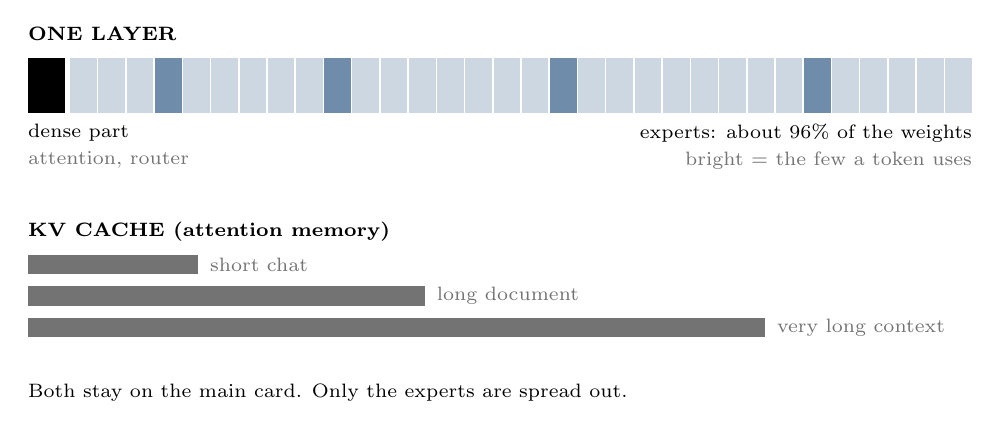
\begin{tikzpicture}
\node[anchor=west, inner sep=0pt, text=black, font=\scriptsize] at (0.000,0.300) {\bfseries ONE LAYER};
\path[fill=black, fill opacity=1.0, draw=none] (0.000,-0.700) rectangle (0.480,0.000);
\path[fill=steelc, fill opacity=0.35, draw=none] (0.540,-0.700) rectangle (0.878,0.000);
\path[fill=steelc, fill opacity=0.35, draw=none] (0.898,-0.700) rectangle (1.237,0.000);
\path[fill=steelc, fill opacity=0.35, draw=none] (1.257,-0.700) rectangle (1.595,0.000);
\path[fill=steelc, fill opacity=1.0, draw=none] (1.615,-0.700) rectangle (1.954,0.000);
\path[fill=steelc, fill opacity=0.35, draw=none] (1.974,-0.700) rectangle (2.312,0.000);
\path[fill=steelc, fill opacity=0.35, draw=none] (2.332,-0.700) rectangle (2.671,0.000);
\path[fill=steelc, fill opacity=0.35, draw=none] (2.691,-0.700) rectangle (3.029,0.000);
\path[fill=steelc, fill opacity=0.35, draw=none] (3.049,-0.700) rectangle (3.387,0.000);
\path[fill=steelc, fill opacity=0.35, draw=none] (3.407,-0.700) rectangle (3.746,0.000);
\path[fill=steelc, fill opacity=1.0, draw=none] (3.766,-0.700) rectangle (4.104,0.000);
\path[fill=steelc, fill opacity=0.35, draw=none] (4.124,-0.700) rectangle (4.463,0.000);
\path[fill=steelc, fill opacity=0.35, draw=none] (4.483,-0.700) rectangle (4.821,0.000);
\path[fill=steelc, fill opacity=0.35, draw=none] (4.841,-0.700) rectangle (5.180,0.000);
\path[fill=steelc, fill opacity=0.35, draw=none] (5.200,-0.700) rectangle (5.538,0.000);
\path[fill=steelc, fill opacity=0.35, draw=none] (5.558,-0.700) rectangle (5.897,0.000);
\path[fill=steelc, fill opacity=0.35, draw=none] (5.917,-0.700) rectangle (6.255,0.000);
\path[fill=steelc, fill opacity=0.35, draw=none] (6.275,-0.700) rectangle (6.613,0.000);
\path[fill=steelc, fill opacity=1.0, draw=none] (6.633,-0.700) rectangle (6.972,0.000);
\path[fill=steelc, fill opacity=0.35, draw=none] (6.992,-0.700) rectangle (7.330,0.000);
\path[fill=steelc, fill opacity=0.35, draw=none] (7.350,-0.700) rectangle (7.689,0.000);
\path[fill=steelc, fill opacity=0.35, draw=none] (7.709,-0.700) rectangle (8.047,0.000);
\path[fill=steelc, fill opacity=0.35, draw=none] (8.067,-0.700) rectangle (8.406,0.000);
\path[fill=steelc, fill opacity=0.35, draw=none] (8.426,-0.700) rectangle (8.764,0.000);
\path[fill=steelc, fill opacity=0.35, draw=none] (8.784,-0.700) rectangle (9.122,0.000);
\path[fill=steelc, fill opacity=0.35, draw=none] (9.142,-0.700) rectangle (9.481,0.000);
\path[fill=steelc, fill opacity=0.35, draw=none] (9.501,-0.700) rectangle (9.839,0.000);
\path[fill=steelc, fill opacity=1.0, draw=none] (9.859,-0.700) rectangle (10.198,0.000);
\path[fill=steelc, fill opacity=0.35, draw=none] (10.218,-0.700) rectangle (10.556,0.000);
\path[fill=steelc, fill opacity=0.35, draw=none] (10.576,-0.700) rectangle (10.915,0.000);
\path[fill=steelc, fill opacity=0.35, draw=none] (10.935,-0.700) rectangle (11.273,0.000);
\path[fill=steelc, fill opacity=0.35, draw=none] (11.293,-0.700) rectangle (11.632,0.000);
\path[fill=steelc, fill opacity=0.35, draw=none] (11.652,-0.700) rectangle (11.990,0.000);
\node[anchor=west, inner sep=0pt, text=black, font=\scriptsize] at (0.000,-0.950) {dense part};
\node[anchor=west, inner sep=0pt, text=black!55, font=\scriptsize] at (0.000,-1.300) {attention, router};
\node[anchor=east, inner sep=0pt, text=black, font=\scriptsize] at (12.000,-0.950) {experts: about 96\% of the weights};
\node[anchor=east, inner sep=0pt, text=black!55, font=\scriptsize] at (12.000,-1.300) {bright = the few a token uses};
\node[anchor=west, inner sep=0pt, text=black, font=\scriptsize] at (0.000,-2.200) {\bfseries KV CACHE (attention memory)};
\path[fill=black, fill opacity=0.55, draw=none] (0.000,-2.750) rectangle (2.160,-2.500);
\node[anchor=west, inner sep=0pt, text=black!55, font=\scriptsize] at (2.310,-2.625) {short chat};
\path[fill=black, fill opacity=0.55, draw=none] (0.000,-3.150) rectangle (5.040,-2.900);
\node[anchor=west, inner sep=0pt, text=black!55, font=\scriptsize] at (5.190,-3.025) {long document};
\path[fill=black, fill opacity=0.55, draw=none] (0.000,-3.550) rectangle (9.360,-3.300);
\node[anchor=west, inner sep=0pt, text=black!55, font=\scriptsize] at (9.510,-3.425) {very long context};
\node[anchor=west, inner sep=0pt, text=black, font=\scriptsize] at (0.000,-4.250) {Both stay on the main card. Only the experts are spread out.};
\end{tikzpicture}

\caption{What a layer weighs (illustrative proportions, not a specific model). The dense part (attention, router,
norms) is small but used by every token, and the KV cache grows with the context; both stay on the main card. The
experts are most of the weight, and a token uses only a few; they are what braiding spreads across cards and RAM.}
\label{fig:weight}
\end{figure}

\section{Expert braiding}
\subsection{Definition}
An MoE layer has a \emph{dense part} (attention, router, norms, sometimes a shared expert) used by every token, and $E$
\emph{experts} of which a token's router picks $k$ (for example $k=8$ of $E=128$). \emph{Expert braiding} assigns the
experts of every layer to devices of different vendors, so that (i) every device holds a slice of every layer's
experts, (ii) each device executes its experts with its own vendor's native kernels in its own process, (iii) the
devices work on the same layer concurrently, and (iv) each (layer, expert) cell has exactly one executing owner at each
placement epoch, so the merged sum is complete and never duplicated. It differs from a layer split, where card A holds
layers $0..29$ and card B holds $30..59$ and the cards take turns.

\subsection{What sits on each card}
The \emph{main card} runs the engine and holds the dense part of every layer and the KV cache, plus a share of each
layer's experts. A \emph{helper card} of another vendor holds another share of each layer's experts, served by a
small helper process built with that vendor's toolkit. A layout holds one main card and up to 62
helpers, 63 cards in all, ordered in \emph{rungs}: the main card is rung 0 and each helper follows in rank order. The
remaining cold experts live in the engine's own tiers, RAM and then NVMe, which form the \emph{fallback rung} below the
cards. Together the rungs form a pyramid (Figure~\ref{fig:racks}), hottest experts at the top. A table kept per layer says
which rung holds which expert; no card holds a whole layer. Which card is main is a choice.

\subsection{One layer, step by step}
Suppose a token at layer 0 was routed to experts 3, 12, 44 and 101.
\begin{enumerate}
\item The engine runs layer 0's attention and router as usual.
\item For each device it builds a batch of the rows whose picks that device owns, masking all other picks
(expert id $-1$, weight zero). Rows whose picks are all masked can be compacted away.
\item The helper's batch (here the rows for experts 12 and 44) goes over shared memory; the main card runs expert 3 and the
engine's fallback runs expert 101 from RAM, all at the same time.
\item Each device returns the weighted sum of the experts it computed.
\item The engine adds the partial outputs to its local experts' output, and moves on to layer 1.
\end{enumerate}
A swap changes only \emph{where} a layer's expert is stored, never its layer: expert 9 of layer 3 means nothing in any
other layer. Each card offers a rack of equal-size slots and a per-layer table says which slot holds which expert, so
a swap trades two experts of the \emph{same} layer. \product{} swaps only between \emph{adjacent card rungs}
(rung $h$ with rung $h+1$), so a hot expert climbs the card ladder one rung per swap toward the main card: for example,
a hot expert on helper 2 swaps with a cold one on helper 1, and later helper 1 swaps with the main card
(Figure~\ref{fig:racks}). With the optional fallback boundary the last helper also swaps with the fallback rung (it loads an expert from the
engine's verified copy and drops a cold one back); the boundary between the main card and the fallback rung stays with the
engine's own adaptive cache (Strata's, in our integration), which moves experts between NVMe, RAM and the main card's cache.

\begin{figure}[t]
\centering
% Generated by gen_figures.py; edit the generator, not this file.
% Copyright 2026 Saltwater Research LLC. SPDX-License-Identifier: Apache-2.0
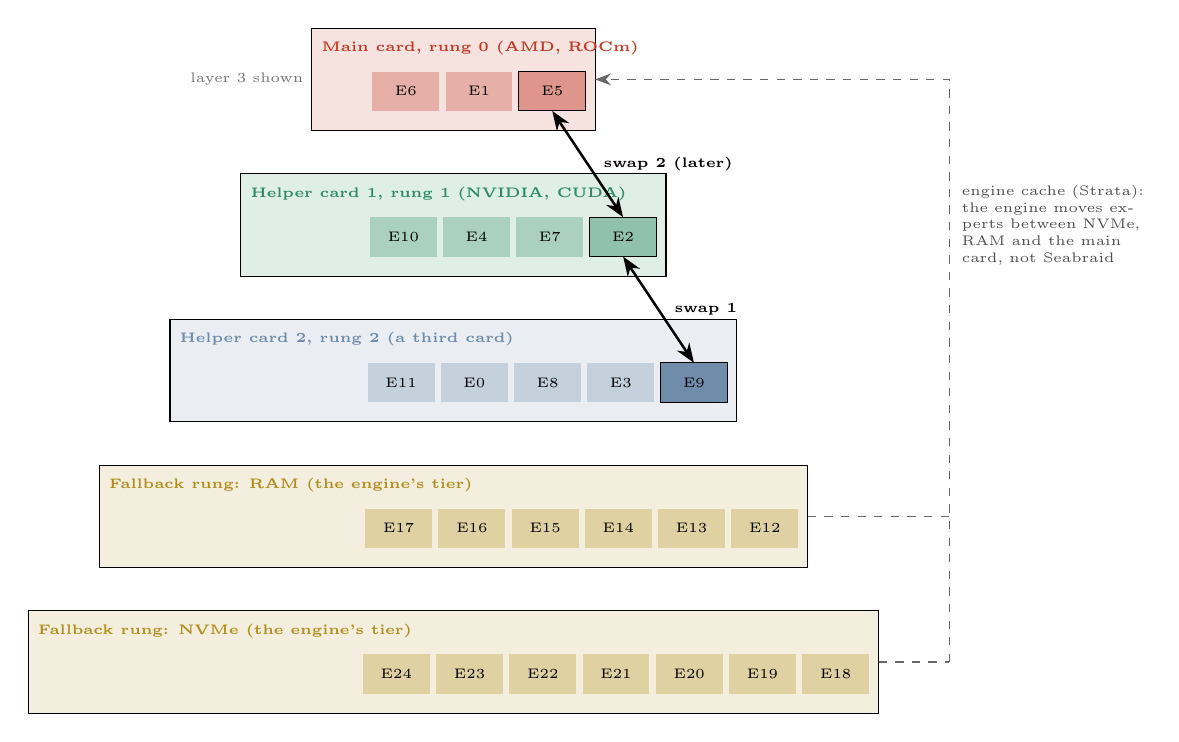
\begin{tikzpicture}
\path[fill=portc, fill opacity=0.15, draw=black, line width=0.4pt] (-1.800,-1.300) rectangle (1.800,0.000);
\node[anchor=west, inner sep=0pt, text=portc, font=\tiny] at (-1.680,-0.250) {\bfseries Main card, rung 0 (AMD, ROCm)};
\path[fill=portc, fill opacity=0.45, draw=black, line width=0.4pt] (0.830,-1.050) rectangle (1.680,-0.550);
\node[anchor=center, inner sep=0pt, text=black, font=\tiny] at (1.255,-0.800) {E5};
\path[fill=portc, fill opacity=0.3, draw=none] (-0.100,-1.050) rectangle (0.750,-0.550);
\node[anchor=center, inner sep=0pt, text=black, font=\tiny] at (0.325,-0.800) {E1};
\path[fill=portc, fill opacity=0.3, draw=none] (-1.030,-1.050) rectangle (-0.180,-0.550);
\node[anchor=center, inner sep=0pt, text=black, font=\tiny] at (-0.605,-0.800) {E6};
\path[fill=stbc, fill opacity=0.15, draw=black, line width=0.4pt] (-2.700,-3.150) rectangle (2.700,-1.850);
\node[anchor=west, inner sep=0pt, text=stbc, font=\tiny] at (-2.580,-2.100) {\bfseries Helper card 1, rung 1 (NVIDIA, CUDA)};
\path[fill=stbc, fill opacity=0.45, draw=black, line width=0.4pt] (1.730,-2.900) rectangle (2.580,-2.400);
\node[anchor=center, inner sep=0pt, text=black, font=\tiny] at (2.155,-2.650) {E2};
\path[fill=stbc, fill opacity=0.3, draw=none] (0.800,-2.900) rectangle (1.650,-2.400);
\node[anchor=center, inner sep=0pt, text=black, font=\tiny] at (1.225,-2.650) {E7};
\path[fill=stbc, fill opacity=0.3, draw=none] (-0.130,-2.900) rectangle (0.720,-2.400);
\node[anchor=center, inner sep=0pt, text=black, font=\tiny] at (0.295,-2.650) {E4};
\path[fill=stbc, fill opacity=0.3, draw=none] (-1.060,-2.900) rectangle (-0.210,-2.400);
\node[anchor=center, inner sep=0pt, text=black, font=\tiny] at (-0.635,-2.650) {E10};
\path[fill=steelc, fill opacity=0.15, draw=black, line width=0.4pt] (-3.600,-5.000) rectangle (3.600,-3.700);
\node[anchor=west, inner sep=0pt, text=steelc, font=\tiny] at (-3.480,-3.950) {\bfseries Helper card 2, rung 2 (a third card)};
\path[fill=steelc, fill opacity=1.0, draw=black, line width=0.4pt] (2.630,-4.750) rectangle (3.480,-4.250);
\node[anchor=center, inner sep=0pt, text=black, font=\tiny] at (3.055,-4.500) {E9};
\path[fill=steelc, fill opacity=0.3, draw=none] (1.700,-4.750) rectangle (2.550,-4.250);
\node[anchor=center, inner sep=0pt, text=black, font=\tiny] at (2.125,-4.500) {E3};
\path[fill=steelc, fill opacity=0.3, draw=none] (0.770,-4.750) rectangle (1.620,-4.250);
\node[anchor=center, inner sep=0pt, text=black, font=\tiny] at (1.195,-4.500) {E8};
\path[fill=steelc, fill opacity=0.3, draw=none] (-0.160,-4.750) rectangle (0.690,-4.250);
\node[anchor=center, inner sep=0pt, text=black, font=\tiny] at (0.265,-4.500) {E0};
\path[fill=steelc, fill opacity=0.3, draw=none] (-1.090,-4.750) rectangle (-0.240,-4.250);
\node[anchor=center, inner sep=0pt, text=black, font=\tiny] at (-0.665,-4.500) {E11};
\path[fill=brassc, fill opacity=0.15, draw=black, line width=0.4pt] (-4.500,-6.850) rectangle (4.500,-5.550);
\node[anchor=west, inner sep=0pt, text=brassc, font=\tiny] at (-4.380,-5.800) {\bfseries Fallback rung: RAM (the engine's tier)};
\path[fill=brassc, fill opacity=0.3, draw=none] (3.530,-6.600) rectangle (4.380,-6.100);
\node[anchor=center, inner sep=0pt, text=black, font=\tiny] at (3.955,-6.350) {E12};
\path[fill=brassc, fill opacity=0.3, draw=none] (2.600,-6.600) rectangle (3.450,-6.100);
\node[anchor=center, inner sep=0pt, text=black, font=\tiny] at (3.025,-6.350) {E13};
\path[fill=brassc, fill opacity=0.3, draw=none] (1.670,-6.600) rectangle (2.520,-6.100);
\node[anchor=center, inner sep=0pt, text=black, font=\tiny] at (2.095,-6.350) {E14};
\path[fill=brassc, fill opacity=0.3, draw=none] (0.740,-6.600) rectangle (1.590,-6.100);
\node[anchor=center, inner sep=0pt, text=black, font=\tiny] at (1.165,-6.350) {E15};
\path[fill=brassc, fill opacity=0.3, draw=none] (-0.190,-6.600) rectangle (0.660,-6.100);
\node[anchor=center, inner sep=0pt, text=black, font=\tiny] at (0.235,-6.350) {E16};
\path[fill=brassc, fill opacity=0.3, draw=none] (-1.120,-6.600) rectangle (-0.270,-6.100);
\node[anchor=center, inner sep=0pt, text=black, font=\tiny] at (-0.695,-6.350) {E17};
\path[fill=brassc, fill opacity=0.15, draw=black, line width=0.4pt] (-5.400,-8.700) rectangle (5.400,-7.400);
\node[anchor=west, inner sep=0pt, text=brassc, font=\tiny] at (-5.280,-7.650) {\bfseries Fallback rung: NVMe (the engine's tier)};
\path[fill=brassc, fill opacity=0.3, draw=none] (4.430,-8.450) rectangle (5.280,-7.950);
\node[anchor=center, inner sep=0pt, text=black, font=\tiny] at (4.855,-8.200) {E18};
\path[fill=brassc, fill opacity=0.3, draw=none] (3.500,-8.450) rectangle (4.350,-7.950);
\node[anchor=center, inner sep=0pt, text=black, font=\tiny] at (3.925,-8.200) {E19};
\path[fill=brassc, fill opacity=0.3, draw=none] (2.570,-8.450) rectangle (3.420,-7.950);
\node[anchor=center, inner sep=0pt, text=black, font=\tiny] at (2.995,-8.200) {E20};
\path[fill=brassc, fill opacity=0.3, draw=none] (1.640,-8.450) rectangle (2.490,-7.950);
\node[anchor=center, inner sep=0pt, text=black, font=\tiny] at (2.065,-8.200) {E21};
\path[fill=brassc, fill opacity=0.3, draw=none] (0.710,-8.450) rectangle (1.560,-7.950);
\node[anchor=center, inner sep=0pt, text=black, font=\tiny] at (1.135,-8.200) {E22};
\path[fill=brassc, fill opacity=0.3, draw=none] (-0.220,-8.450) rectangle (0.630,-7.950);
\node[anchor=center, inner sep=0pt, text=black, font=\tiny] at (0.205,-8.200) {E23};
\path[fill=brassc, fill opacity=0.3, draw=none] (-1.150,-8.450) rectangle (-0.300,-7.950);
\node[anchor=center, inner sep=0pt, text=black, font=\tiny] at (-0.725,-8.200) {E24};
\draw[{Stealth}-{Stealth}, line width=0.9pt] (3.055,-4.250) -- (2.155,-2.900);
\node[anchor=west, inner sep=0pt, text=black, font=\tiny] at (2.805,-3.575) {\bfseries swap 1};
\draw[{Stealth}-{Stealth}, line width=0.9pt] (2.155,-2.400) -- (1.255,-1.050);
\node[anchor=west, inner sep=0pt, text=black, font=\tiny] at (1.905,-1.725) {\bfseries swap 2 (later)};
\draw[dashed, line width=0.6pt, black!60] (4.500,-6.200) -- (6.300,-6.200);
\draw[dashed, line width=0.6pt, black!60] (5.400,-8.050) -- (6.300,-8.050);
\draw[dashed, -{Stealth}, line width=0.6pt, black!60] (6.300,-8.050) -- (6.300,-0.650) -- (1.800,-0.650);
\node[anchor=west, inner sep=0pt, text width=2.4cm, font=\tiny, text=black!70] at (6.450,-2.500) {engine cache (Strata): the engine moves experts between NVMe, RAM and the main card, not \product};
\node[anchor=east, inner sep=0pt, text=black!55, font=\tiny] at (-1.900,-0.650) {layer 3 shown};
\end{tikzpicture}

\caption{The placement pyramid for one layer (layer 3 is drawn; every layer has the same shape). Rung 0 is the main
card, then helper cards in rank order (up to 63 cards in all; three are drawn), then the fallback rung (RAM, then NVMe,
the engine's own tiers). Solid arrows are \product's live swaps: always the same layer, always between adjacent card
rungs. Swap~1 trades hot expert 9 on helper 2 with cold expert 2 on helper 1; swap~2 later trades that expert with
one on the main card. Each swap is staged, acknowledged by the card and published under a new epoch. Dashed arrows
are the engine's own cache (Strata) moving experts between NVMe, RAM and the main card; \product{} does not do that.
The optional fallback boundary, not drawn here, adds swaps between the last helper and the fallback rung
(Figure~\ref{fig:pyramid-live}). Schematic, not to scale.}
\label{fig:racks}
\end{figure}

\section{System design}
\begin{figure}[t]
\centering
% Copyright 2026 Saltwater Research LLC. SPDX-License-Identifier: Apache-2.0
% System diagram (hand-written; plain TikZ, arrows.meta only). Schematic.
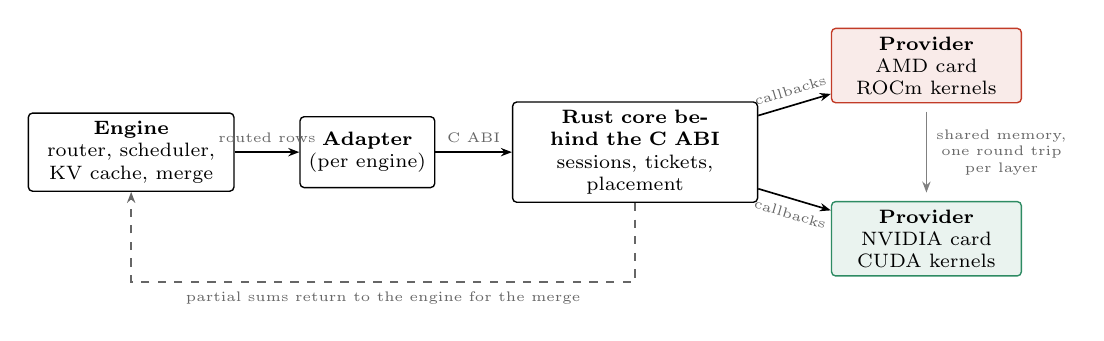
\begin{tikzpicture}[
  box/.style={draw, rounded corners=1.5pt, align=center, font=\scriptsize, inner sep=3pt, minimum height=0.9cm, line width=0.5pt},
  arr/.style={-{Stealth[length=4pt]}, line width=0.6pt},
  lab/.style={font=\tiny, text=black!60, align=center}]
\node[box, text width=2.4cm] (eng) at (0,0) {\textbf{Engine}\\router, scheduler,\\KV cache, merge};
\node[box, text width=1.5cm] (adp) at (3.0,0) {\textbf{Adapter}\\(per engine)};
\node[box, text width=2.9cm] (core) at (6.4,0) {\textbf{Rust core behind the C ABI}\\sessions, tickets,\\placement};
\node[box, text width=2.2cm, draw=portc, fill=portc!10] (cb) at (10.1,1.1) {\textbf{Provider}\\AMD card\\ROCm kernels};
\node[box, text width=2.2cm, draw=stbc, fill=stbc!10] (cc) at (10.1,-1.1) {\textbf{Provider}\\NVIDIA card\\CUDA kernels};
\draw[arr] (eng) -- node[above, lab] {routed rows} (adp);
\draw[arr] (adp) -- node[above, lab] {C ABI} (core);
\draw[arr] (core) -- node[above, lab, sloped] {callbacks} (cb);
\draw[arr] (core) -- node[below, lab, sloped] {callbacks} (cc);
\draw[arr, black!50] ([yshift=-3pt]cb.south) -- node[right, lab] {shared memory,\\one round trip\\per layer} ([yshift=3pt]cc.north);
\draw[arr, dashed, black!60] (core.south) -- ++(0,-1.0) -| node[below, lab, pos=0.25] {partial sums return to the engine for the merge} (eng.south);
\end{tikzpicture}

\caption{System overview. The engine keeps loading, routing, scheduling, KV state and the final merge. The Rust core
owns sessions, tickets, buffers, validation and placement bookkeeping. Providers execute a batch on one device with
native kernels; in the Strata adapter each provider talks to a per-vendor helper process over shared memory.
Schematic.}
\label{fig:system}
\end{figure}

Figure~\ref{fig:system} shows the parts. The core opens no sockets and uses no network; a provider and an adapter see only validated, copied batches.

\paragraph{C ABI.} The ABI has sessions with a single in-flight ticket; provider callbacks v1 (one operation) and v2 (a
dense table of operations on one worker, with a partial-routes flag); capability discovery and activation provenance
tags; status counters; a log sink, last-error query and version string; and the placement API. Calls copy their
inputs. Layout compatibility is carried by a layout epoch and the SONAME; appends ride on a \texttt{struct\_size}
field. The ABI is alpha and may change before 1.0.

\paragraph{Sessions, tickets and partial routes.} A session owns one dedicated worker thread and one in-flight batch.
A submit returns a ticket that the engine later collects. A batch may carry only some of a row's picks (a partial
route): the others carry the skip id with weight zero, and the provider returns a partial sum.

\paragraph{Helper processes.} For cards of different vendors, the Strata adapter launches a helper process
per card (a design choice, see the introduction) and exchanges batches through a shared-memory channel. The controller passes a sealed memory descriptor to the helper
(no named mapping), validates its identity and geometry, and starts a pidfd watcher so the helper exits if the
controller dies without teardown. A helper that fails or times out is retired, and later requests route locally.
There is no network and no peer-to-peer transfer. Two copies of the activations cross the handoff; no faster path has been measured.

\paragraph{Acknowledged live placement.} Placement binds one engine model layout to a Rust ownership map (a port of
the ownership map that our add-on patch 0012 adds to Strata) and a heat planner.
A layout holds 1 to 63 cards, and the fallback rung is the one after the last card.
\emph{Fill} is hottest-first spillover: the lead card (rung 0) fills first, then each helper card in rung order (rank
order from the ranking helper), and the remainder goes to the fallback rung, the engine's own tiers (RAM, then NVMe).
\emph{Plan} proposes same-layer exchanges only between adjacent card rungs: it visits the boundaries from the top
(rung 0 against rung 1 first), promotes a hot expert from rung $h+1$ into rung $h$ and displaces the coldest resident
one, subject to a promotion margin (a challenger needs more than a set multiple of the incumbent's smoothed heat), a
per-layer helper-share ceiling, a cooldown and a per-round move budget; a cell moves at most once per round, so a hot
expert climbs the ladder one rung per swap. The fallback rung never takes part in a live swap. Planning performs no
provider work. \emph{Apply}: the engine stops admission and drains
in-flight work, then \product{} runs stage and replace callbacks and commits ownership only on acknowledgement.
\emph{Publish}: the new executor table and its epoch are published at the same fence, so no batch is routed against a
half-applied swap, and a batch carrying a stale epoch is refused.

\paragraph{Failure contract.} A refusal changes nothing. A failed write restores the known slot. Uncertain completion
quarantines the card, whose cells route to the fallback. A helper that dies fails the in-flight request and later
requests are served locally. A wrong expert never runs silently.

\paragraph{Safety.} The Rust core owns every lifetime rule. The FFI tests run under Miri in both aliasing models,
Stacked Borrows and Tree Borrows, in continuous integration; Miri found real undefined behaviour in an earlier handle
gate, fixed by changing the handle's memory layout without changing the C ABI, and now reports none. The native tests also run
under AddressSanitizer and UndefinedBehaviorSanitizer (Table~\ref{tab:runtime}).

\section{Implementation}
The core is Rust. Engines connect through adapters over the C ABI. The Strata adapter, with a patch series for a
pinned Strata source tree and the original add-on, was the first to run live. The ggml adapter provides a prepared-graph
cache and an opt-in llama.cpp hook; it ran a synthetic Q4\_0 fixture on CPU, CUDA, HIP and Vulkan against ggml 1.0.0.
Python bindings expose the same runtime for adoption and testing. A provider callback can be as small as 21 lines of C (100 lines with its driver).
Supported cards on the Strata path are bounded by Strata's kernels (NVIDIA sm\_80 and newer; AMD RDNA3 and RDNA4).

\section{Evaluation}
All results are from one machine class and are \emph{not} general benchmarks. Every figure is one run ($n=1$) unless a
count is given. Superscript tags name the record in the repository that holds the setup: RL followed by a month-day is
the entry of that date in the project's research log (11-17b is its second 2026-11-17 entry); AO is the add-on's
results table and design log; ABI is the ABI reference. Figures not written down in the repository are not
reproduced here.

\subsection{Earlier Strata add-on}
The first measurements use the add-on to Strata, whose helper mechanism \product{}
generalizes. They are \emph{not} measurements of the \product{} runtime. Model: Qwen3.8-Flash-Next (GSQ-RCO quants)
unless stated; measured 2026-11-06 and 2026-11-07 (Table~\ref{tab:addon}).

\begin{table}[t]
\centering\footnotesize
\begin{tabular}{@{}p{3.6cm}p{3.4cm}p{7.2cm}@{}}
\toprule
Setup & Hardware & Result\\
\midrule
Strata alone, IQ2\_XS\rl{AO} & RTX 3090 + RTX 3060; R9700 alone & 113.4 tok/s e2e; 98.6 tok/s. Expert cache 99.8\% hit, so a second card adds nothing for this model\\
Add-on, model fits (expert cap 11,000)\rl{AO} & R9700 32 GB + RTX 3060 & 95.9 vs 96.0 tok/s e2e (stock): a tie\\
Add-on, model does not fit (cap 4,000)\rl{AO} & same & 8 of 10 classification prompts answered at about 70 tok/s decode; stock 0 of 10 (hung); stock greedy 52--60 tok/s\\
IQ3\_S, all in VRAM\rl{AO} & R9700 32 GB + RTX 3090 24 GB (PCIe 3.0 x8, 280 W cap) & 105.5 / 106.0 / 105.6 (tiered config) and 105.9 / 105.9 / 105.6 tok/s (all-VRAM), 3 runs of 2,000 greedy tokens, wall time\\
IQ3\_S, tiered, for comparison\rl{AO} & R9700 + RTX 3060 & 96--99 tok/s\\
Per-card expert throughput, IQ3\_S layer 24, 200 decode iterations\rl{AO} & R9700 / RTX 3090, both capped at 250 W & 268,572 / 230,744 decode rows/s\\
DeepSeek-V4.1-Flash, 128 tokens, one 32-token prompt (historical; measured 2026-11-07 on Strata 0.1.58, add-on build c9823b0)\rl{AO} & R9700 + RTX 3090 & 10.08 tok/s with the add-on vs 6.17 tok/s stock, same session\\
Teacher-forced KL, 441 positions, mean top-32\rl{AO} & R9700 + RTX 3060 & stock vs stock 0.0025; add-on vs stock 0.0098 (top-1 agreement 96.1\%)\\
\bottomrule
\end{tabular}
\caption{Add-on measurements (Strata, earlier mechanism). $n=1$ each unless stated.}
\label{tab:addon}
\end{table}

Caveats. (i) The two 3090 configurations agree because the RAM budget in the tiered configuration placed
0 bytes; the gain over the 3060 setup came from the card swap, not from tiering. An earlier prediction of +3--9\% was
retracted. (ii) The DeepSeek speed-up is, per an independent review, I/O relief: the 3090 acts as a 22.8 GiB cache in
front of slower storage, and more host RAM would likely do the same. (iii) The DeepSeek KL gate \textbf{failed}
its thresholds and was noise-dominated. Perplexity was +3.0\% and +3.6\% above stock on two segments, and the review calls
the gap real on paired statistics. It is open and unexplained, and the DeepSeek path should not be relied on for output
quality. (iv) The hot-share option is opt-in and off: the helper's time per request roughly doubled, and the per-window
gain is inside run-to-run drift. (v) The payoff evidence is two measured points, not a threshold: with the model fitting on the main card
(cap 11,000) the add-on tied stock (95.9 vs 96.0 tok/s), and at cap 4,000 it completed 8 of 10 classification prompts
against 0 of 10 for stock, which is a different metric and workload. No paired, repeated sweep was run.

\subsection{The \product{} runtime}
Host class for every live run: one Linux x86-64 machine with an AMD R9700 (HIP, gfx1201) and an NVIDIA RTX 3090
(CUDA, sm\_86). Engine: Strata v0.2.15 unless stated. Table~\ref{tab:live} lists the live runs and Table~\ref{tab:runtime} the test gates.

\begin{table}[t]
\centering\footnotesize
\begin{tabular}{@{}p{3.3cm}p{2.4cm}p{8.5cm}@{}}
\toprule
Test & Date & Result\\
\midrule
Live decode, previous pin (Strata v0.2.13.1)\rl{RL 11-16} & 2026-11-16 & 89.5 to 95.0 tok/s greedy decode over six runs\\
Live decode, IQ3\_S, 2,000 greedy tokens, $n=6$ per arm\rl{RL 11-17} & 2026-11-17 & R9700 main + 3090 helper: mean 94.8 tok/s (sd 3.0, range 91.1--98.4; 94.75 on the previous pin). 3090 main + R9700 helper: mean 106.7 (sd 2.0, range 104.6--110.2; 16,000 helper slots)\\
Helper SIGKILL, 3 per arm, fresh engine each\rl{RL 11-17} & 2026-11-17 & Request failed after 0.33--0.46 s (HIP main) and 0.51--0.73 s (CUDA main); next request served 1.7--1.8 s and 2.5--2.7 s after the kill; no zombie. Earlier pin 11-16: client error after 0.33--0.44 s\\
KL quality gate against the main card alone, both card orders, 3 short texts, 1 engine start per arm\rl{RL 11-17} & 2026-11-17 & Pooled result passed in both orders (thresholds: $\mathrm{KL}\le 0.03$, top-1 $\ge 0.95$). The KL and top-1 values were not recorded\\
Long prompts, private helper tier (before $\to$ after a fix)\rl{RL 11-17b} & 2026-11-17 & First token at 32k tokens 32.0--35.7 s $\to$ 20.3 and 18.0 s; 128k 135.5 $\to$ 80.7 s; 261k 260--269 $\to$ about 128 s; needles found; short-prompt decode 91.8--98.5 $\to$ 91.8--98.4 tok/s. No change with the 3090 as main. Run count not recorded\\
Live pyramid L1: three boundaries, capped capacity (Figure~\ref{fig:pyramid-live})\rl{RL 11-19} & 2026-11-19 & 1,539 moves in 513 rounds all committed and verified; decode-path KL 0.0013 against the main card alone (gate 0.03). Helper loss failed (see text)\\
Live pyramid L2: one expert through every level, and file-reference moves\rl{RL 11-20} & 2026-11-20 & One cell (layer 39, expert 16) made all eight transitions in 428 rounds; file-reference run: 744 moves in 248 rounds, none non-committed, 124 hops by file reference; decode-path KL 0.00116 and 0.00121 against a floor of 0.00116 (gate 0.03)\\
D4 remote prefill (opt-in), $n=2$ per mode\rl{RL 11-17} & 2026-11-17 & Engaged, but an 8.3k-token prompt read slower than lending; off by default\\
llama.cpp hook logit parity, 2,044 positions over 4 texts\rl{RL 11-17/18} & 2026-11-17/18 & Bit-identical to stock on CPU, CUDA, HIP, and a Vulkan layer split. The hook does not call the runtime, so this is \emph{not} an expert split\\
\bottomrule
\end{tabular}
\caption{Live results of the \product{} runtime on one machine. Strata v0.2.15 unless stated.}
\label{tab:live}
\end{table}

\begin{table}[t]
\centering\footnotesize
\begin{tabular}{@{}p{4.6cm}p{2.2cm}p{7.4cm}@{}}
\toprule
Gate & Date & Result\\
\midrule
Rust tests; CTest; ASan+UBSan\rl{RL 11-16} & 2026-11-16 & 53 of 53; 13 of 13 (8 without the Strata adapter); 8 of 8\\
Strata ctest on the patched tree\rl{RL 11-17} & 2026-11-17 & CPU 138 pass / 0 fail; HIP 291 / 2; CUDA 357 / 2 (a missing model, and two that fail on a pristine tree too)\\
Seabraid CTest; Rust\rl{RL 11-17} & 2026-11-17 & 16 of 16 in Release and ASan+UBSan; 62 Rust tests\\
Seabraid CTest; Rust\rl{RL 11-18} & 2026-11-18 & 19 of 19 in Release and ASan+UBSan; 63 of 63\\
FFI tests under Miri (both models)\rl{ABI} & 2026-11-19 & No undefined behaviour reported under Stacked Borrows and Tree Borrows; Miri sees only what the tests exercise, so this is a diagnostic, not a proof of memory safety\\
ggml fixture (Q4\_0), ggml 1.0.0\rl{RL 11-14, 11-17} & 2026-11-17 & Passes on CPU, CUDA, HIP and Vulkan; the deliberate cache miss failed the regression\\
\bottomrule
\end{tabular}
\caption{Test gates of the runtime (counts as written in the log on each date).}
\label{tab:runtime}
\end{table}

\paragraph{Negative and open results.} The first live-placement run (2026-11-18, matched arms, 2 to 4 engine starts per
cell, Strata v0.2.15) was \emph{not a pass}.\rl{RL 11-18} Mean decode, which includes the stalls, did not pass. Pauses of 10 s or more in
the archived W1 arms (counts as recorded by the independent audit of 2026-11-19, out of 12 per arm) were: private live
3, private static 0, zero-move control 0, named new publisher 2, named legacy 1, named static 1; run-wide 15 of 194
promotion requests against 5 of 140 static or control requests. Recomputed request means were 93.66 tok/s for private
static and 75.66 tok/s for private live. Whether the moves or host memory pressure (pinned expert RAM leaves about
285 MiB free) cause the difference is unproven and needs a comparison that varies RAM headroom and promotion separately.
Live promotion therefore stays experimental and opt-in, and static placement is the supported baseline. Placement never settles at the
default margin and interval; one KL text sits at about $4\times$ its noise floor after moves; and the 100 ms fence
budget is provisional. The per-arm figures were not written into the repository and are not reproduced. No
speed-up over stock has been shown for the new runtime.

\subsection{Live pyramid (L1)}
This run exercises the placement pyramid on real cards: a main card and two helpers, with rung F
holding the experts the cards could not.\rl{RL 11-19} Setup, as in Figure~\ref{fig:pyramid-live}: one machine; main card an
R9700 (HIP); helper 1 an RTX 3090 (CUDA); helper 2 a second HIP helper \emph{process} on the same R9700, not a third card; rung F
is the engine's RAM (6 GiB budget) plus NVMe. Model Qwen3.8-Flash-Next IQ3\_S with capped capacity (2,582, 1,500 and 1,000 expert
slots on the three cards), so 66\% of the 24,576 experts lived on NVMe, and the page cache was evicted so SSD reads were real.
Revision: the repository at commit e9cc304 and the Strata v7 patch series.

\paragraph{Placement.} Under natural traffic (scenario S2) all 1,539 moves in 513 rounds committed with
\texttt{verified=1}, with no stale-epoch refusal, and every move carried exactly the pack's per-layer blob size. Moves per
boundary are in Figure~\ref{fig:l1-moves}: 520 between main and helper 1, 481 between helpers 1 and 2, 538 between helper 2 and
rung F (an equal number down). Of the 538 promotions from rung F, 413 were read from the engine's RAM and 125 from the SSD pack
file. In a second run with heat steered to force a full descent (S6), expert 407 of layer 25 (2,329,600 bytes) climbed from the
SSD file to helper 2, helper 1 and the main card in round 7, then was pushed down to helper 1 (round 290), helper 2 (round 333)
and rung F, landing on the SSD only (round 388), verified at each hop. The placement round fence averaged 18.7 ms (99th
percentile 52 ms), about 1.2\% of the time between rounds; this is one run, not a measured budget.

\paragraph{Quality.} Decode-path KL against the main card alone, over 2,400 positions from six texts and two separate engine
starts of the pyramid: KL 0.00132 and 0.00130, top-1 agreement 0.9817 and 0.9858, against a noise floor (a second main-card-alone
run) of 0.00135 and 0.985; both passed the gate ($\mathrm{KL}\le 0.03$, top-1 $\ge 0.95$).

\paragraph{Failed and not exercised.} Two successive helper losses \textbf{failed}: a killed named helper stalled decode for
30 s and the engine then exited (HTTP 400, then 503); helper loss was not survived by named channel helpers in that run. A re-run after two fixes (runs HL and HL2, 2026-11-20) is described below (HL, HL2). Run L1 did not exercise file-reference moves (see L2 below), compaction, a third physical card or a live trace file. Decode ran at 4.2 to
7.8 tok/s under deliberate SSD starvation and load from other work; this is \emph{not} a performance claim and not a comparison
with static placement.

\paragraph{Live run L2 (2026-11-20).} Same layout, built from commit f423da7 with Strata patches 0001 to 0018 and the v7 patch.
One expert (layer 39, expert 16) made all eight transitions in one run of 428 rounds and 7 requests: SSD to RAM (round 28; the page
cache was dropped to 20,480 bytes and the 1,971,200-byte read took 2,761 $\mu$s), RAM to helper 2, helper 2 to helper 1 to main
(round 79, \texttt{verified=1}), main to helper 1 (118), helper 1 to helper 2 (176), helper 2 to RAM (274) and RAM to SSD only
(278). Seven of 14 steered cells made all eight. The scenario had 1,281 committed moves, 3 non-committed and 0 stale epochs.
File-reference moves ran on the GPUs in a second scenario: 744 moves in 248 rounds, none non-committed, 124 hops by file reference
(48 from F to helper 2, 76 from helper 2 to helper 1) and 190 by bytes; helper file io 256,307,200 direct bytes in 372 reads,
\texttt{bad\_sum=0}. By-reference writes were 2.6 to 3.0 times slower than byte writes, because the helper reads the NVMe itself;
the main card's stage time was 12 to 15\% lower. Decode-path KL with file moves live, over 2,400 positions (six texts, top-32): 0.00116
(top-1 0.9904) and 0.00121 (top-1 0.9871) against a noise floor of 0.00116; both passed the gate. Round cost was 28.8 ms mean
(p99 54.8) and 35.2 ms (p99 56.6). \texttt{verified=1} covers the card-to-card hops; the two hops that touch the fallback log
\texttt{verified=0} by design, and that the bytes came off the drive is inferred from the page-cache drop and the 2.76 ms read, not
from a block-level trace. The RAM install and eviction were driven by a real switch of request type, because the RAM copy follows
real routing. Compaction with the pyramid was not run: its flag acts only on the private helper tier, which has one helper. Decode
ran at 1.9 to 4.8 tok/s at box load 8 to 23, which is load-contaminated, not a performance figure.

\begin{figure}[t]
\centering
% Generated by gen_live_l2.py; edit the generator, not this file.
% Copyright 2026 Saltwater Research LLC. SPDX-License-Identifier: Apache-2.0
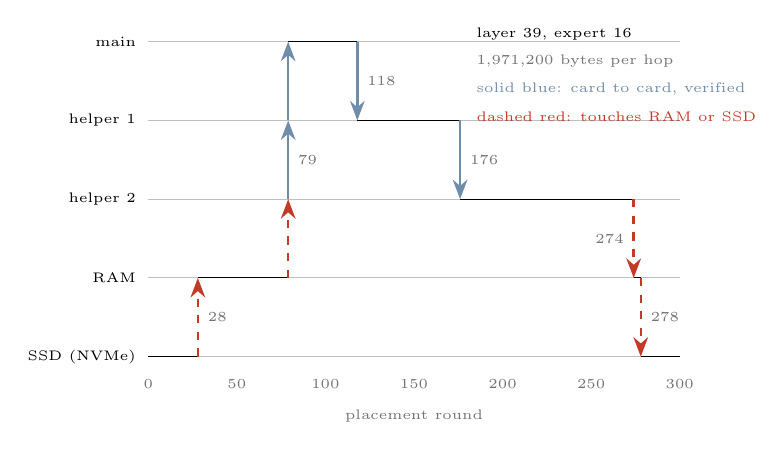
\begin{tikzpicture}
\draw[line width=0.4pt, draw=black!25] (0.000,0.000) -- (6.750,0.000);
\node[anchor=east, inner sep=0pt, text=black, font=\tiny] at (-0.150,0.000) {main};
\draw[line width=0.4pt, draw=black!25] (0.000,-1.000) -- (6.750,-1.000);
\node[anchor=east, inner sep=0pt, text=black, font=\tiny] at (-0.150,-1.000) {helper 1};
\draw[line width=0.4pt, draw=black!25] (0.000,-2.000) -- (6.750,-2.000);
\node[anchor=east, inner sep=0pt, text=black, font=\tiny] at (-0.150,-2.000) {helper 2};
\draw[line width=0.4pt, draw=black!25] (0.000,-3.000) -- (6.750,-3.000);
\node[anchor=east, inner sep=0pt, text=black, font=\tiny] at (-0.150,-3.000) {RAM};
\draw[line width=0.4pt, draw=black!25] (0.000,-4.000) -- (6.750,-4.000);
\node[anchor=east, inner sep=0pt, text=black, font=\tiny] at (-0.150,-4.000) {SSD (NVMe)};
\node[anchor=center, inner sep=0pt, text=black!55, font=\tiny] at (0.000,-4.350) {0};
\node[anchor=center, inner sep=0pt, text=black!55, font=\tiny] at (1.125,-4.350) {50};
\node[anchor=center, inner sep=0pt, text=black!55, font=\tiny] at (2.250,-4.350) {100};
\node[anchor=center, inner sep=0pt, text=black!55, font=\tiny] at (3.375,-4.350) {150};
\node[anchor=center, inner sep=0pt, text=black!55, font=\tiny] at (4.500,-4.350) {200};
\node[anchor=center, inner sep=0pt, text=black!55, font=\tiny] at (5.625,-4.350) {250};
\node[anchor=center, inner sep=0pt, text=black!55, font=\tiny] at (6.750,-4.350) {300};
\node[anchor=center, inner sep=0pt, text=black!55, font=\tiny] at (3.375,-4.750) {placement round};
\draw[line width=0.4pt, draw=black] (0.000,-4.000) -- (0.630,-4.000);
\draw[line width=0.4pt, draw=black] (0.630,-3.000) -- (1.777,-3.000);
\draw[line width=0.4pt, draw=black] (1.777,-2.000) -- (1.777,-2.000);
\draw[line width=0.4pt, draw=black] (1.777,-1.000) -- (1.777,-1.000);
\draw[line width=0.4pt, draw=black] (1.777,0.000) -- (2.655,0.000);
\draw[line width=0.4pt, draw=black] (2.655,-1.000) -- (3.960,-1.000);
\draw[line width=0.4pt, draw=black] (3.960,-2.000) -- (6.165,-2.000);
\draw[line width=0.4pt, draw=black] (6.165,-3.000) -- (6.255,-3.000);
\draw[line width=0.4pt, draw=black] (6.255,-4.000) -- (6.750,-4.000);
\draw[dashed, -{Stealth}, line width=0.9pt, draw=portc] (0.630,-4.000) -- (0.630,-3.000);
\draw[dashed, -{Stealth}, line width=0.9pt, draw=portc] (1.777,-3.000) -- (1.777,-2.000);
\draw[-{Stealth}, line width=0.9pt, draw=steelc] (1.777,-2.000) -- (1.777,-1.000);
\draw[-{Stealth}, line width=0.9pt, draw=steelc] (1.777,-1.000) -- (1.777,0.000);
\draw[-{Stealth}, line width=0.9pt, draw=steelc] (2.655,0.000) -- (2.655,-1.000);
\draw[-{Stealth}, line width=0.9pt, draw=steelc] (3.960,-1.000) -- (3.960,-2.000);
\draw[dashed, -{Stealth}, line width=0.9pt, draw=portc] (6.165,-2.000) -- (6.165,-3.000);
\draw[dashed, -{Stealth}, line width=0.9pt, draw=portc] (6.255,-3.000) -- (6.255,-4.000);
\node[anchor=west, inner sep=0pt, text=black!55, font=\tiny] at (0.750,-3.500) {28};
\node[anchor=west, inner sep=0pt, text=black!55, font=\tiny] at (1.897,-1.500) {79};
\node[anchor=west, inner sep=0pt, text=black!55, font=\tiny] at (2.775,-0.500) {118};
\node[anchor=west, inner sep=0pt, text=black!55, font=\tiny] at (4.080,-1.500) {176};
\node[anchor=east, inner sep=0pt, text=black!55, font=\tiny] at (6.045,-2.500) {274};
\node[anchor=west, inner sep=0pt, text=black!55, font=\tiny] at (6.375,-3.500) {278};
\node[anchor=west, inner sep=0pt, text=black, font=\tiny] at (4.162,0.100) {layer 39, expert 16};
\node[anchor=west, inner sep=0pt, text=black!55, font=\tiny] at (4.162,-0.250) {1,971,200 bytes per hop};
\node[anchor=west, inner sep=0pt, text=steelc, font=\tiny] at (4.162,-0.600) {solid blue: card to card, verified};
\node[anchor=west, inner sep=0pt, text=portc, font=\tiny] at (4.162,-0.950) {dashed red: touches RAM or SSD};
\end{tikzpicture}

\caption{Live run L2, same machine as L1: one expert (layer 39, expert 16, 1,971,200 bytes) at each placement round, from the SSD
through RAM, helper 2, helper 1 and the main card and back. Solid arrows are card-to-card hops (\texttt{verified=1}); dashed arrows
touch RAM or the SSD and are \texttt{verified=0} by design. Schematic, not to scale in the levels.}
\label{fig:l2-walk}
\end{figure}

\paragraph{Helper loss on GPUs (runs HL and HL2, 2026-11-20).} Same machine and layout; HL ran commit f04173e (patches 0001 to 0019 and the v7 patch), HL2 the code with patch 0020. A helper killed mid-request: 7 of 7 requests succeeded in each run, with one engine start, and the dead helper's card closed 22 to 93 ms after the kill while the request in flight finished. A helper killed while idle: 4 of 4 later requests succeeded; the card closes at the next layer request, 34 to 203 ms into it, not at the kill. Restart with both helpers dead: ready in 34 to 35 s with one warning per card after a SIGKILL of the engine. After a graceful engine stop the restart \textbf{failed} in HL (the engine exited, ``not ready for a plan (state 5)'') because the channel state was read before the helper's identity; patch 0020 binds the identity first, so a dead helper opens its card closed whatever the state, and in HL2 the restart was ready in 32 s with 6 of 6 requests succeeding. A restart while a live helper is still in its shutdown state (the engine waits for it for at most 30 s) has a CPU test only. Machine load was 4 to 14, so no timing is a performance figure.

\begin{figure}[t]
\centering
% Generated by gen_live_figures.py; edit the generator, not this file.
% Copyright 2026 Saltwater Research LLC. SPDX-License-Identifier: Apache-2.0
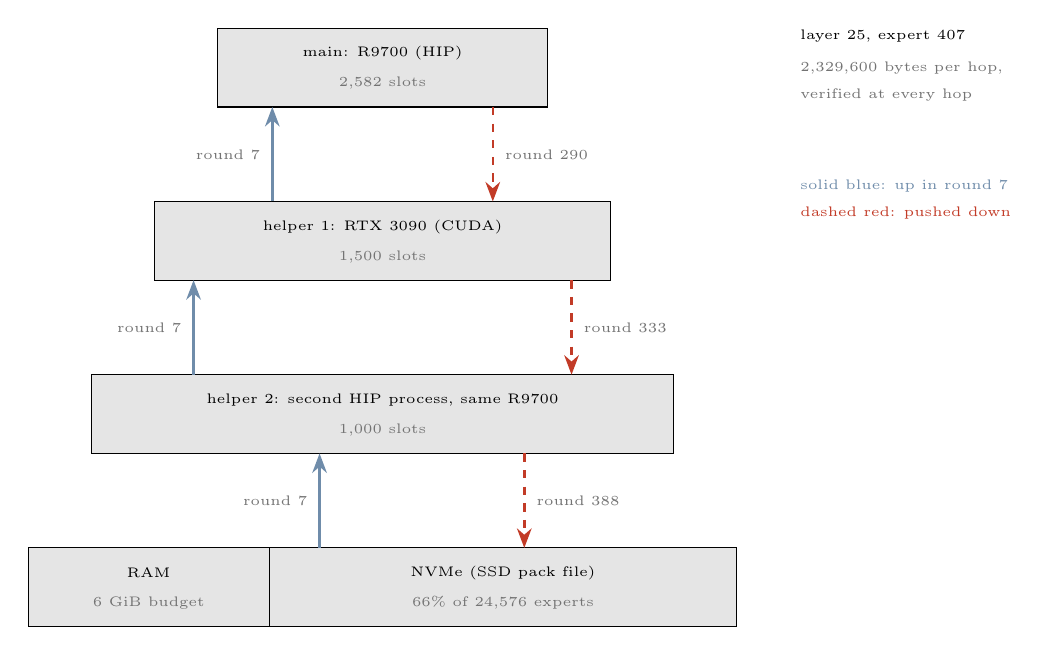
\begin{tikzpicture}
\path[fill=black!25, fill opacity=0.4, draw=black, line width=0.4pt] (-2.100,-1.000) rectangle (2.100,0.000);
\node[anchor=center, inner sep=0pt, text=black, font=\tiny] at (0.000,-0.320) {main: R9700 (HIP)};
\node[anchor=center, inner sep=0pt, text=black!55, font=\tiny] at (0.000,-0.700) {2,582 slots};
\path[fill=black!25, fill opacity=0.4, draw=black, line width=0.4pt] (-2.900,-3.200) rectangle (2.900,-2.200);
\node[anchor=center, inner sep=0pt, text=black, font=\tiny] at (0.000,-2.520) {helper 1: RTX 3090 (CUDA)};
\node[anchor=center, inner sep=0pt, text=black!55, font=\tiny] at (0.000,-2.900) {1,500 slots};
\path[fill=black!25, fill opacity=0.4, draw=black, line width=0.4pt] (-3.700,-5.400) rectangle (3.700,-4.400);
\node[anchor=center, inner sep=0pt, text=black, font=\tiny] at (0.000,-4.720) {helper 2: second HIP process, same R9700};
\node[anchor=center, inner sep=0pt, text=black!55, font=\tiny] at (0.000,-5.100) {1,000 slots};
\path[fill=black!25, fill opacity=0.4, draw=black, line width=0.4pt] (-4.500,-7.600) rectangle (4.500,-6.600);
\draw[line width=0.4pt] (-1.440,-6.600) -- (-1.440,-7.600);
\node[anchor=center, inner sep=0pt, text=black, font=\tiny] at (-2.970,-6.920) {RAM};
\node[anchor=center, inner sep=0pt, text=black!55, font=\tiny] at (-2.970,-7.300) {6 GiB budget};
\node[anchor=center, inner sep=0pt, text=black, font=\tiny] at (1.530,-6.920) {NVMe (SSD pack file)};
\node[anchor=center, inner sep=0pt, text=black!55, font=\tiny] at (1.530,-7.300) {66\% of 24,576 experts};
\draw[-{Stealth}, line width=0.9pt, draw=steelc] (-0.800,-6.600) -- (-0.800,-5.400);
\node[anchor=east, inner sep=0pt, text=black!55, font=\tiny] at (-0.950,-6.000) {round 7};
\draw[-{Stealth}, line width=0.9pt, draw=steelc] (-2.400,-4.400) -- (-2.400,-3.200);
\node[anchor=east, inner sep=0pt, text=black!55, font=\tiny] at (-2.550,-3.800) {round 7};
\draw[-{Stealth}, line width=0.9pt, draw=steelc] (-1.400,-2.200) -- (-1.400,-1.000);
\node[anchor=east, inner sep=0pt, text=black!55, font=\tiny] at (-1.550,-1.600) {round 7};
\draw[dashed, -{Stealth}, line width=0.9pt, draw=portc] (1.400,-1.000) -- (1.400,-2.200);
\node[anchor=west, inner sep=0pt, text=black!55, font=\tiny] at (1.550,-1.600) {round 290};
\draw[dashed, -{Stealth}, line width=0.9pt, draw=portc] (2.400,-3.200) -- (2.400,-4.400);
\node[anchor=west, inner sep=0pt, text=black!55, font=\tiny] at (2.550,-3.800) {round 333};
\draw[dashed, -{Stealth}, line width=0.9pt, draw=portc] (1.800,-5.400) -- (1.800,-6.600);
\node[anchor=west, inner sep=0pt, text=black!55, font=\tiny] at (1.950,-6.000) {round 388};
\node[anchor=west, inner sep=0pt, text=black, font=\tiny] at (5.300,-0.100) {layer 25, expert 407};
\node[anchor=west, inner sep=0pt, text=black!55, font=\tiny] at (5.300,-0.500) {2,329,600 bytes per hop,};
\node[anchor=west, inner sep=0pt, text=black!55, font=\tiny] at (5.300,-0.850) {verified at every hop};
\node[anchor=west, inner sep=0pt, text=steelc, font=\tiny] at (5.300,-2.000) {solid blue: up in round 7};
\node[anchor=west, inner sep=0pt, text=portc, font=\tiny] at (5.300,-2.350) {dashed red: pushed down};
\end{tikzpicture}

\caption{Live run L1, one machine: main card R9700 (HIP), helper 1 RTX 3090 (CUDA), helper 2 a second HIP process on the same
R9700 (not a third card), rung F the engine's RAM plus NVMe; capped capacity, 66\% of 24,576 experts on NVMe. Expert 407 of layer
25 climbed in round 7 (solid) and was pushed down in rounds 290, 333 and 388 (dashed), each hop 2,329,600 bytes, verified.
Schematic, not to scale.}
\label{fig:pyramid-live}
\end{figure}

\begin{figure}[t]
\centering
% Generated by gen_live_figures.py; edit the generator, not this file.
% Copyright 2026 Saltwater Research LLC. SPDX-License-Identifier: Apache-2.0
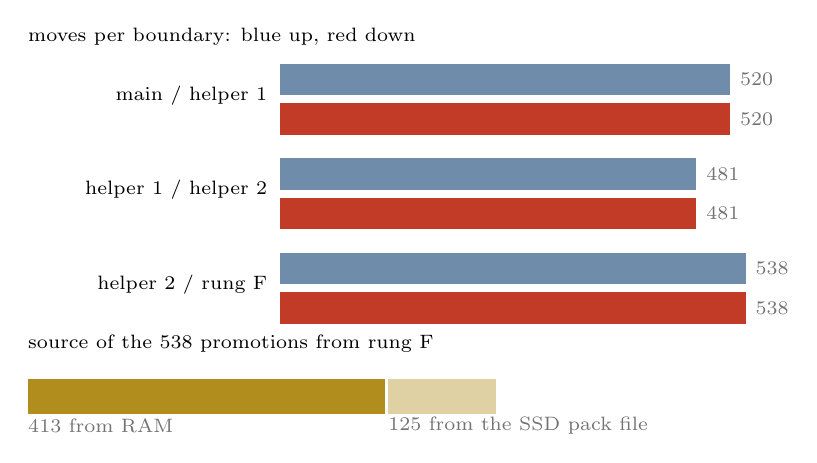
\begin{tikzpicture}
\node[anchor=west, inner sep=0pt, text=black, font=\scriptsize] at (0.000,0.350) {moves per boundary: blue up, red down};
\node[anchor=east, inner sep=0pt, text=black, font=\scriptsize] at (3.050,-0.400) {main / helper 1};
\path[fill=steelc, fill opacity=1.0, draw=none] (3.200,-0.400) rectangle (8.920,0.000);
\node[anchor=west, inner sep=0pt, text=black!55, font=\scriptsize] at (9.040,-0.200) {520};
\path[fill=portc, fill opacity=1.0, draw=none] (3.200,-0.900) rectangle (8.920,-0.500);
\node[anchor=west, inner sep=0pt, text=black!55, font=\scriptsize] at (9.040,-0.700) {520};
\node[anchor=east, inner sep=0pt, text=black, font=\scriptsize] at (3.050,-1.600) {helper 1 / helper 2};
\path[fill=steelc, fill opacity=1.0, draw=none] (3.200,-1.600) rectangle (8.491,-1.200);
\node[anchor=west, inner sep=0pt, text=black!55, font=\scriptsize] at (8.611,-1.400) {481};
\path[fill=portc, fill opacity=1.0, draw=none] (3.200,-2.100) rectangle (8.491,-1.700);
\node[anchor=west, inner sep=0pt, text=black!55, font=\scriptsize] at (8.611,-1.900) {481};
\node[anchor=east, inner sep=0pt, text=black, font=\scriptsize] at (3.050,-2.800) {helper 2 / rung F};
\path[fill=steelc, fill opacity=1.0, draw=none] (3.200,-2.800) rectangle (9.118,-2.400);
\node[anchor=west, inner sep=0pt, text=black!55, font=\scriptsize] at (9.238,-2.600) {538};
\path[fill=portc, fill opacity=1.0, draw=none] (3.200,-3.300) rectangle (9.118,-2.900);
\node[anchor=west, inner sep=0pt, text=black!55, font=\scriptsize] at (9.238,-3.100) {538};
\node[anchor=west, inner sep=0pt, text=black, font=\scriptsize] at (0.000,-3.550) {source of the 538 promotions from rung F};
\path[fill=brassc, fill opacity=1.0, draw=none] (0.000,-4.450) rectangle (4.543,-4.000);
\path[fill=brassc, fill opacity=0.4, draw=none] (4.573,-4.450) rectangle (5.948,-4.000);
\node[anchor=west, inner sep=0pt, text=black!55, font=\scriptsize] at (0.000,-4.600) {413 from RAM};
\node[anchor=west, inner sep=0pt, text=black!55, font=\scriptsize] at (4.573,-4.600) {125 from the SSD pack file};
\end{tikzpicture}

\caption{Live run L1, natural traffic: 1,539 committed moves in 513 rounds, per boundary and direction, and the source of the
538 promotions from rung F (413 from RAM, 125 from the SSD pack file). Same machine and capacity as Figure~\ref{fig:pyramid-live}.}
\label{fig:l1-moves}
\end{figure}

Figure~\ref{fig:archs} sets expert braiding beside the architectures it is usually compared with.

\begin{figure*}[t]
\centering
% Generated by gen_figures.py; edit the generator, not this file.
% Copyright 2026 Saltwater Research LLC. SPDX-License-Identifier: Apache-2.0
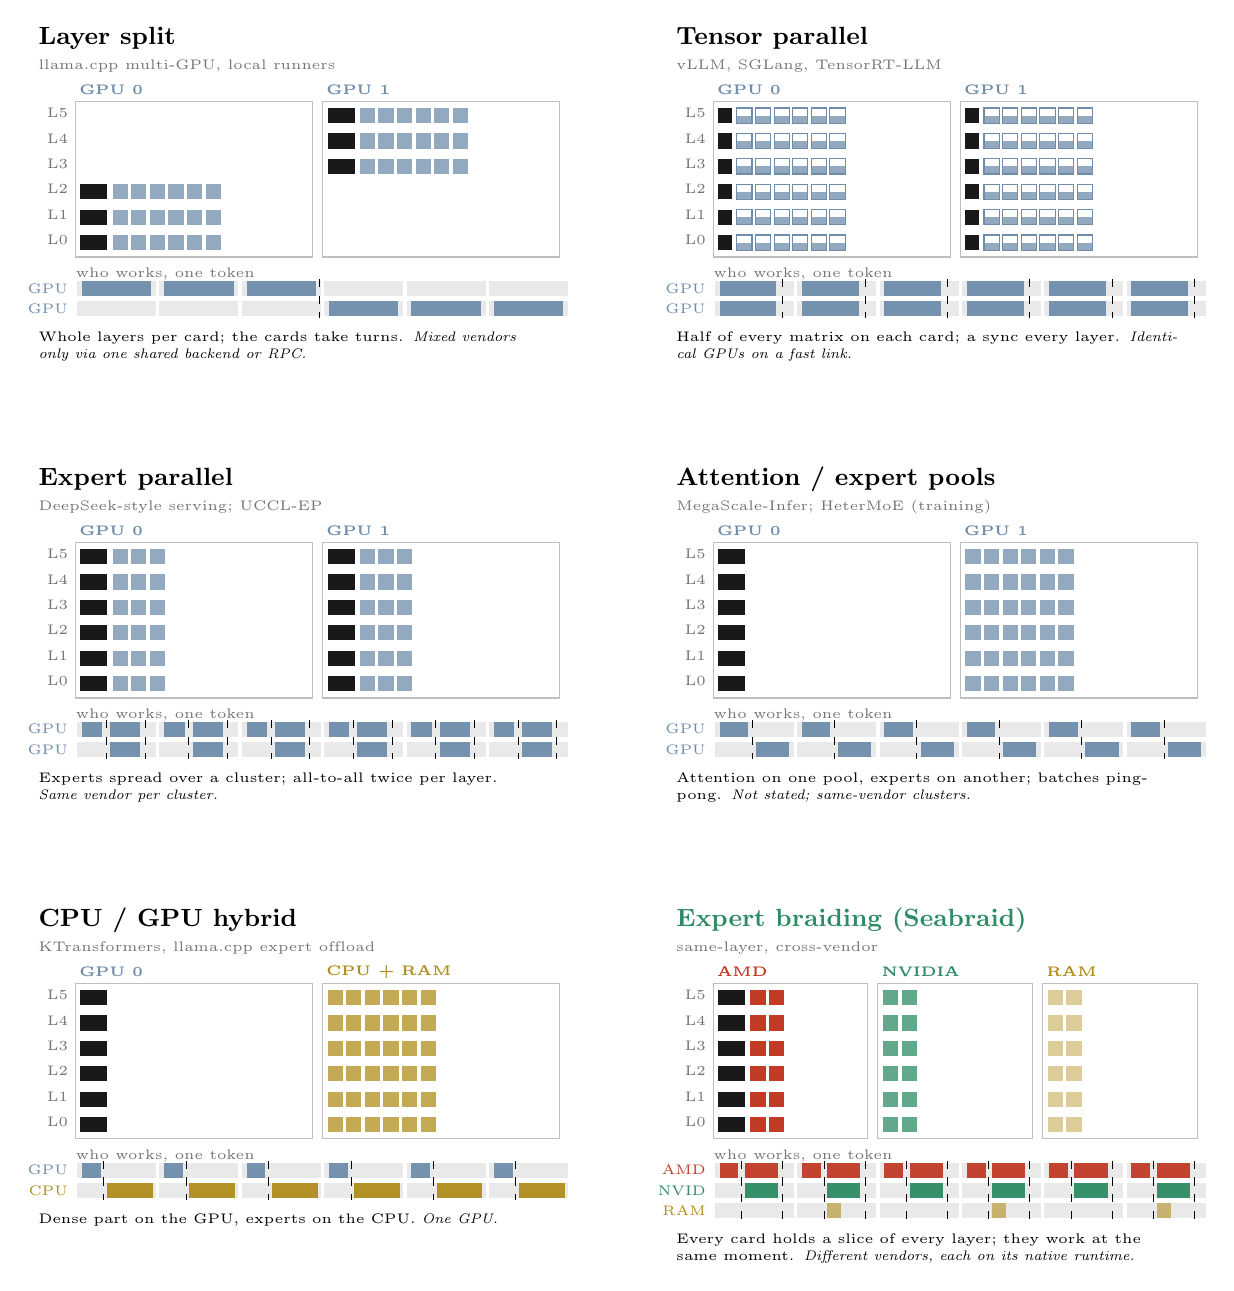
\begin{tikzpicture}
\begin{scope}[shift={(0.000,0.000)}]
\node[anchor=west, inner sep=0pt, text=black, font=\small] at (0.000,0.450) {\bfseries Layer split};
\node[anchor=west, inner sep=0pt, text=black!55, font=\tiny] at (0.000,0.100) {llama.cpp multi-GPU, local runners};
\node[anchor=west, inner sep=0pt, text=steelc, font=\tiny] at (0.516,-0.200) {\bfseries GPU 0};
\path[draw=black!25, line width=0.4pt] (0.473,-2.322) rectangle (3.483,-0.344);
\node[anchor=west, inner sep=0pt, text=steelc, font=\tiny] at (3.655,-0.200) {\bfseries GPU 1};
\path[draw=black!25, line width=0.4pt] (3.612,-2.322) rectangle (6.622,-0.344);
\node[anchor=east, inner sep=0pt, text=black!55, font=\tiny] at (0.387,-2.107) {L0};
\path[fill=black, fill opacity=0.9, draw=none] (0.537,-2.236) rectangle (0.881,-2.042);
\path[fill=steelc, fill opacity=0.75, draw=none] (0.946,-2.236) rectangle (1.139,-2.042);
\path[fill=steelc, fill opacity=0.75, draw=none] (1.182,-2.236) rectangle (1.376,-2.042);
\path[fill=steelc, fill opacity=0.75, draw=none] (1.419,-2.236) rectangle (1.612,-2.042);
\path[fill=steelc, fill opacity=0.75, draw=none] (1.655,-2.236) rectangle (1.849,-2.042);
\path[fill=steelc, fill opacity=0.75, draw=none] (1.892,-2.236) rectangle (2.085,-2.042);
\path[fill=steelc, fill opacity=0.75, draw=none] (2.128,-2.236) rectangle (2.322,-2.042);
\node[anchor=east, inner sep=0pt, text=black!55, font=\tiny] at (0.387,-1.784) {L1};
\path[fill=black, fill opacity=0.9, draw=none] (0.537,-1.913) rectangle (0.881,-1.720);
\path[fill=steelc, fill opacity=0.75, draw=none] (0.946,-1.913) rectangle (1.139,-1.720);
\path[fill=steelc, fill opacity=0.75, draw=none] (1.182,-1.913) rectangle (1.376,-1.720);
\path[fill=steelc, fill opacity=0.75, draw=none] (1.419,-1.913) rectangle (1.612,-1.720);
\path[fill=steelc, fill opacity=0.75, draw=none] (1.655,-1.913) rectangle (1.849,-1.720);
\path[fill=steelc, fill opacity=0.75, draw=none] (1.892,-1.913) rectangle (2.085,-1.720);
\path[fill=steelc, fill opacity=0.75, draw=none] (2.128,-1.913) rectangle (2.322,-1.720);
\node[anchor=east, inner sep=0pt, text=black!55, font=\tiny] at (0.387,-1.462) {L2};
\path[fill=black, fill opacity=0.9, draw=none] (0.537,-1.591) rectangle (0.881,-1.397);
\path[fill=steelc, fill opacity=0.75, draw=none] (0.946,-1.591) rectangle (1.139,-1.397);
\path[fill=steelc, fill opacity=0.75, draw=none] (1.182,-1.591) rectangle (1.376,-1.397);
\path[fill=steelc, fill opacity=0.75, draw=none] (1.419,-1.591) rectangle (1.612,-1.397);
\path[fill=steelc, fill opacity=0.75, draw=none] (1.655,-1.591) rectangle (1.849,-1.397);
\path[fill=steelc, fill opacity=0.75, draw=none] (1.892,-1.591) rectangle (2.085,-1.397);
\path[fill=steelc, fill opacity=0.75, draw=none] (2.128,-1.591) rectangle (2.322,-1.397);
\node[anchor=east, inner sep=0pt, text=black!55, font=\tiny] at (0.387,-1.139) {L3};
\path[fill=black, fill opacity=0.9, draw=none] (3.676,-1.268) rectangle (4.021,-1.075);
\path[fill=steelc, fill opacity=0.75, draw=none] (4.085,-1.268) rectangle (4.279,-1.075);
\path[fill=steelc, fill opacity=0.75, draw=none] (4.321,-1.268) rectangle (4.515,-1.075);
\path[fill=steelc, fill opacity=0.75, draw=none] (4.558,-1.268) rectangle (4.752,-1.075);
\path[fill=steelc, fill opacity=0.75, draw=none] (4.794,-1.268) rectangle (4.988,-1.075);
\path[fill=steelc, fill opacity=0.75, draw=none] (5.031,-1.268) rectangle (5.224,-1.075);
\path[fill=steelc, fill opacity=0.75, draw=none] (5.267,-1.268) rectangle (5.461,-1.075);
\node[anchor=east, inner sep=0pt, text=black!55, font=\tiny] at (0.387,-0.817) {L4};
\path[fill=black, fill opacity=0.9, draw=none] (3.676,-0.946) rectangle (4.021,-0.752);
\path[fill=steelc, fill opacity=0.75, draw=none] (4.085,-0.946) rectangle (4.279,-0.752);
\path[fill=steelc, fill opacity=0.75, draw=none] (4.321,-0.946) rectangle (4.515,-0.752);
\path[fill=steelc, fill opacity=0.75, draw=none] (4.558,-0.946) rectangle (4.752,-0.752);
\path[fill=steelc, fill opacity=0.75, draw=none] (4.794,-0.946) rectangle (4.988,-0.752);
\path[fill=steelc, fill opacity=0.75, draw=none] (5.031,-0.946) rectangle (5.224,-0.752);
\path[fill=steelc, fill opacity=0.75, draw=none] (5.267,-0.946) rectangle (5.461,-0.752);
\node[anchor=east, inner sep=0pt, text=black!55, font=\tiny] at (0.387,-0.494) {L5};
\path[fill=black, fill opacity=0.9, draw=none] (3.676,-0.623) rectangle (4.021,-0.430);
\path[fill=steelc, fill opacity=0.75, draw=none] (4.085,-0.623) rectangle (4.279,-0.430);
\path[fill=steelc, fill opacity=0.75, draw=none] (4.321,-0.623) rectangle (4.515,-0.430);
\path[fill=steelc, fill opacity=0.75, draw=none] (4.558,-0.623) rectangle (4.752,-0.430);
\path[fill=steelc, fill opacity=0.75, draw=none] (4.794,-0.623) rectangle (4.988,-0.430);
\path[fill=steelc, fill opacity=0.75, draw=none] (5.031,-0.623) rectangle (5.224,-0.430);
\path[fill=steelc, fill opacity=0.75, draw=none] (5.267,-0.623) rectangle (5.461,-0.430);
\node[anchor=west, inner sep=0pt, text=black!55, font=\tiny] at (0.473,-2.537) {who works, one token};
\node[anchor=east, inner sep=0pt, text=steelc, font=\tiny] at (0.387,-2.720) {GPU};
\node[anchor=east, inner sep=0pt, text=steelc, font=\tiny] at (0.387,-2.978) {GPU};
\path[fill=black!25, fill opacity=0.35, draw=none] (0.494,-2.816) rectangle (1.498,-2.623);
\path[fill=black!25, fill opacity=0.35, draw=none] (0.494,-3.074) rectangle (1.498,-2.881);
\path[fill=steelc, fill opacity=0.95, draw=none] (0.555,-2.816) rectangle (1.438,-2.623);
\path[fill=black!25, fill opacity=0.35, draw=none] (1.541,-2.816) rectangle (2.544,-2.623);
\path[fill=black!25, fill opacity=0.35, draw=none] (1.541,-3.074) rectangle (2.544,-2.881);
\path[fill=steelc, fill opacity=0.95, draw=none] (1.601,-2.816) rectangle (2.484,-2.623);
\path[fill=black!25, fill opacity=0.35, draw=none] (2.587,-2.816) rectangle (3.590,-2.623);
\path[fill=black!25, fill opacity=0.35, draw=none] (2.587,-3.074) rectangle (3.590,-2.881);
\path[fill=steelc, fill opacity=0.95, draw=none] (2.647,-2.816) rectangle (3.530,-2.623);
\draw[dashed, line width=0.3pt] (3.570,-2.601) -- (3.570,-3.096);
\path[fill=black!25, fill opacity=0.35, draw=none] (3.633,-2.816) rectangle (4.637,-2.623);
\path[fill=black!25, fill opacity=0.35, draw=none] (3.633,-3.074) rectangle (4.637,-2.881);
\path[fill=steelc, fill opacity=0.95, draw=none] (3.694,-3.074) rectangle (4.577,-2.881);
\path[fill=black!25, fill opacity=0.35, draw=none] (4.680,-2.816) rectangle (5.683,-2.623);
\path[fill=black!25, fill opacity=0.35, draw=none] (4.680,-3.074) rectangle (5.683,-2.881);
\path[fill=steelc, fill opacity=0.95, draw=none] (4.740,-3.074) rectangle (5.623,-2.881);
\path[fill=black!25, fill opacity=0.35, draw=none] (5.726,-2.816) rectangle (6.729,-2.623);
\path[fill=black!25, fill opacity=0.35, draw=none] (5.726,-3.074) rectangle (6.729,-2.881);
\path[fill=steelc, fill opacity=0.95, draw=none] (5.786,-3.074) rectangle (6.669,-2.881);
\node[anchor=north west, inner sep=0pt, text width=6.41cm, font=\tiny] at (0,-3.268) {Whole layers per card; the cards take turns. \emph{Mixed vendors only via one shared backend or RPC.}};
\end{scope}
\begin{scope}[shift={(8.100,0.000)}]
\node[anchor=west, inner sep=0pt, text=black, font=\small] at (0.000,0.450) {\bfseries Tensor parallel};
\node[anchor=west, inner sep=0pt, text=black!55, font=\tiny] at (0.000,0.100) {vLLM, SGLang, TensorRT-LLM};
\node[anchor=west, inner sep=0pt, text=steelc, font=\tiny] at (0.516,-0.200) {\bfseries GPU 0};
\path[draw=black!25, line width=0.4pt] (0.473,-2.322) rectangle (3.483,-0.344);
\node[anchor=west, inner sep=0pt, text=steelc, font=\tiny] at (3.655,-0.200) {\bfseries GPU 1};
\path[draw=black!25, line width=0.4pt] (3.612,-2.322) rectangle (6.622,-0.344);
\node[anchor=east, inner sep=0pt, text=black!55, font=\tiny] at (0.387,-2.107) {L0};
\path[fill=black, fill opacity=0.9, draw=none] (0.537,-2.236) rectangle (0.710,-2.042);
\path[draw=steelc, line width=0.4pt] (0.774,-2.236) rectangle (0.967,-2.042);
\path[fill=steelc, fill opacity=0.75, draw=none] (0.774,-2.236) rectangle (0.967,-2.139);
\path[draw=steelc, line width=0.4pt] (1.010,-2.236) rectangle (1.204,-2.042);
\path[fill=steelc, fill opacity=0.75, draw=none] (1.010,-2.236) rectangle (1.204,-2.139);
\path[draw=steelc, line width=0.4pt] (1.247,-2.236) rectangle (1.440,-2.042);
\path[fill=steelc, fill opacity=0.75, draw=none] (1.247,-2.236) rectangle (1.440,-2.139);
\path[draw=steelc, line width=0.4pt] (1.483,-2.236) rectangle (1.677,-2.042);
\path[fill=steelc, fill opacity=0.75, draw=none] (1.483,-2.236) rectangle (1.677,-2.139);
\path[draw=steelc, line width=0.4pt] (1.720,-2.236) rectangle (1.913,-2.042);
\path[fill=steelc, fill opacity=0.75, draw=none] (1.720,-2.236) rectangle (1.913,-2.139);
\path[draw=steelc, line width=0.4pt] (1.956,-2.236) rectangle (2.150,-2.042);
\path[fill=steelc, fill opacity=0.75, draw=none] (1.956,-2.236) rectangle (2.150,-2.139);
\path[fill=black, fill opacity=0.9, draw=none] (3.676,-2.236) rectangle (3.849,-2.042);
\path[draw=steelc, line width=0.4pt] (3.913,-2.236) rectangle (4.106,-2.042);
\path[fill=steelc, fill opacity=0.75, draw=none] (3.913,-2.236) rectangle (4.106,-2.139);
\path[draw=steelc, line width=0.4pt] (4.149,-2.236) rectangle (4.343,-2.042);
\path[fill=steelc, fill opacity=0.75, draw=none] (4.149,-2.236) rectangle (4.343,-2.139);
\path[draw=steelc, line width=0.4pt] (4.386,-2.236) rectangle (4.579,-2.042);
\path[fill=steelc, fill opacity=0.75, draw=none] (4.386,-2.236) rectangle (4.579,-2.139);
\path[draw=steelc, line width=0.4pt] (4.622,-2.236) rectangle (4.816,-2.042);
\path[fill=steelc, fill opacity=0.75, draw=none] (4.622,-2.236) rectangle (4.816,-2.139);
\path[draw=steelc, line width=0.4pt] (4.859,-2.236) rectangle (5.053,-2.042);
\path[fill=steelc, fill opacity=0.75, draw=none] (4.859,-2.236) rectangle (5.053,-2.139);
\path[draw=steelc, line width=0.4pt] (5.095,-2.236) rectangle (5.289,-2.042);
\path[fill=steelc, fill opacity=0.75, draw=none] (5.095,-2.236) rectangle (5.289,-2.139);
\node[anchor=east, inner sep=0pt, text=black!55, font=\tiny] at (0.387,-1.784) {L1};
\path[fill=black, fill opacity=0.9, draw=none] (0.537,-1.913) rectangle (0.710,-1.720);
\path[draw=steelc, line width=0.4pt] (0.774,-1.913) rectangle (0.967,-1.720);
\path[fill=steelc, fill opacity=0.75, draw=none] (0.774,-1.913) rectangle (0.967,-1.817);
\path[draw=steelc, line width=0.4pt] (1.010,-1.913) rectangle (1.204,-1.720);
\path[fill=steelc, fill opacity=0.75, draw=none] (1.010,-1.913) rectangle (1.204,-1.817);
\path[draw=steelc, line width=0.4pt] (1.247,-1.913) rectangle (1.440,-1.720);
\path[fill=steelc, fill opacity=0.75, draw=none] (1.247,-1.913) rectangle (1.440,-1.817);
\path[draw=steelc, line width=0.4pt] (1.483,-1.913) rectangle (1.677,-1.720);
\path[fill=steelc, fill opacity=0.75, draw=none] (1.483,-1.913) rectangle (1.677,-1.817);
\path[draw=steelc, line width=0.4pt] (1.720,-1.913) rectangle (1.913,-1.720);
\path[fill=steelc, fill opacity=0.75, draw=none] (1.720,-1.913) rectangle (1.913,-1.817);
\path[draw=steelc, line width=0.4pt] (1.956,-1.913) rectangle (2.150,-1.720);
\path[fill=steelc, fill opacity=0.75, draw=none] (1.956,-1.913) rectangle (2.150,-1.817);
\path[fill=black, fill opacity=0.9, draw=none] (3.676,-1.913) rectangle (3.849,-1.720);
\path[draw=steelc, line width=0.4pt] (3.913,-1.913) rectangle (4.106,-1.720);
\path[fill=steelc, fill opacity=0.75, draw=none] (3.913,-1.913) rectangle (4.106,-1.817);
\path[draw=steelc, line width=0.4pt] (4.149,-1.913) rectangle (4.343,-1.720);
\path[fill=steelc, fill opacity=0.75, draw=none] (4.149,-1.913) rectangle (4.343,-1.817);
\path[draw=steelc, line width=0.4pt] (4.386,-1.913) rectangle (4.579,-1.720);
\path[fill=steelc, fill opacity=0.75, draw=none] (4.386,-1.913) rectangle (4.579,-1.817);
\path[draw=steelc, line width=0.4pt] (4.622,-1.913) rectangle (4.816,-1.720);
\path[fill=steelc, fill opacity=0.75, draw=none] (4.622,-1.913) rectangle (4.816,-1.817);
\path[draw=steelc, line width=0.4pt] (4.859,-1.913) rectangle (5.053,-1.720);
\path[fill=steelc, fill opacity=0.75, draw=none] (4.859,-1.913) rectangle (5.053,-1.817);
\path[draw=steelc, line width=0.4pt] (5.095,-1.913) rectangle (5.289,-1.720);
\path[fill=steelc, fill opacity=0.75, draw=none] (5.095,-1.913) rectangle (5.289,-1.817);
\node[anchor=east, inner sep=0pt, text=black!55, font=\tiny] at (0.387,-1.462) {L2};
\path[fill=black, fill opacity=0.9, draw=none] (0.537,-1.591) rectangle (0.710,-1.397);
\path[draw=steelc, line width=0.4pt] (0.774,-1.591) rectangle (0.967,-1.397);
\path[fill=steelc, fill opacity=0.75, draw=none] (0.774,-1.591) rectangle (0.967,-1.494);
\path[draw=steelc, line width=0.4pt] (1.010,-1.591) rectangle (1.204,-1.397);
\path[fill=steelc, fill opacity=0.75, draw=none] (1.010,-1.591) rectangle (1.204,-1.494);
\path[draw=steelc, line width=0.4pt] (1.247,-1.591) rectangle (1.440,-1.397);
\path[fill=steelc, fill opacity=0.75, draw=none] (1.247,-1.591) rectangle (1.440,-1.494);
\path[draw=steelc, line width=0.4pt] (1.483,-1.591) rectangle (1.677,-1.397);
\path[fill=steelc, fill opacity=0.75, draw=none] (1.483,-1.591) rectangle (1.677,-1.494);
\path[draw=steelc, line width=0.4pt] (1.720,-1.591) rectangle (1.913,-1.397);
\path[fill=steelc, fill opacity=0.75, draw=none] (1.720,-1.591) rectangle (1.913,-1.494);
\path[draw=steelc, line width=0.4pt] (1.956,-1.591) rectangle (2.150,-1.397);
\path[fill=steelc, fill opacity=0.75, draw=none] (1.956,-1.591) rectangle (2.150,-1.494);
\path[fill=black, fill opacity=0.9, draw=none] (3.676,-1.591) rectangle (3.849,-1.397);
\path[draw=steelc, line width=0.4pt] (3.913,-1.591) rectangle (4.106,-1.397);
\path[fill=steelc, fill opacity=0.75, draw=none] (3.913,-1.591) rectangle (4.106,-1.494);
\path[draw=steelc, line width=0.4pt] (4.149,-1.591) rectangle (4.343,-1.397);
\path[fill=steelc, fill opacity=0.75, draw=none] (4.149,-1.591) rectangle (4.343,-1.494);
\path[draw=steelc, line width=0.4pt] (4.386,-1.591) rectangle (4.579,-1.397);
\path[fill=steelc, fill opacity=0.75, draw=none] (4.386,-1.591) rectangle (4.579,-1.494);
\path[draw=steelc, line width=0.4pt] (4.622,-1.591) rectangle (4.816,-1.397);
\path[fill=steelc, fill opacity=0.75, draw=none] (4.622,-1.591) rectangle (4.816,-1.494);
\path[draw=steelc, line width=0.4pt] (4.859,-1.591) rectangle (5.053,-1.397);
\path[fill=steelc, fill opacity=0.75, draw=none] (4.859,-1.591) rectangle (5.053,-1.494);
\path[draw=steelc, line width=0.4pt] (5.095,-1.591) rectangle (5.289,-1.397);
\path[fill=steelc, fill opacity=0.75, draw=none] (5.095,-1.591) rectangle (5.289,-1.494);
\node[anchor=east, inner sep=0pt, text=black!55, font=\tiny] at (0.387,-1.139) {L3};
\path[fill=black, fill opacity=0.9, draw=none] (0.537,-1.268) rectangle (0.710,-1.075);
\path[draw=steelc, line width=0.4pt] (0.774,-1.268) rectangle (0.967,-1.075);
\path[fill=steelc, fill opacity=0.75, draw=none] (0.774,-1.268) rectangle (0.967,-1.172);
\path[draw=steelc, line width=0.4pt] (1.010,-1.268) rectangle (1.204,-1.075);
\path[fill=steelc, fill opacity=0.75, draw=none] (1.010,-1.268) rectangle (1.204,-1.172);
\path[draw=steelc, line width=0.4pt] (1.247,-1.268) rectangle (1.440,-1.075);
\path[fill=steelc, fill opacity=0.75, draw=none] (1.247,-1.268) rectangle (1.440,-1.172);
\path[draw=steelc, line width=0.4pt] (1.483,-1.268) rectangle (1.677,-1.075);
\path[fill=steelc, fill opacity=0.75, draw=none] (1.483,-1.268) rectangle (1.677,-1.172);
\path[draw=steelc, line width=0.4pt] (1.720,-1.268) rectangle (1.913,-1.075);
\path[fill=steelc, fill opacity=0.75, draw=none] (1.720,-1.268) rectangle (1.913,-1.172);
\path[draw=steelc, line width=0.4pt] (1.956,-1.268) rectangle (2.150,-1.075);
\path[fill=steelc, fill opacity=0.75, draw=none] (1.956,-1.268) rectangle (2.150,-1.172);
\path[fill=black, fill opacity=0.9, draw=none] (3.676,-1.268) rectangle (3.849,-1.075);
\path[draw=steelc, line width=0.4pt] (3.913,-1.268) rectangle (4.106,-1.075);
\path[fill=steelc, fill opacity=0.75, draw=none] (3.913,-1.268) rectangle (4.106,-1.172);
\path[draw=steelc, line width=0.4pt] (4.149,-1.268) rectangle (4.343,-1.075);
\path[fill=steelc, fill opacity=0.75, draw=none] (4.149,-1.268) rectangle (4.343,-1.172);
\path[draw=steelc, line width=0.4pt] (4.386,-1.268) rectangle (4.579,-1.075);
\path[fill=steelc, fill opacity=0.75, draw=none] (4.386,-1.268) rectangle (4.579,-1.172);
\path[draw=steelc, line width=0.4pt] (4.622,-1.268) rectangle (4.816,-1.075);
\path[fill=steelc, fill opacity=0.75, draw=none] (4.622,-1.268) rectangle (4.816,-1.172);
\path[draw=steelc, line width=0.4pt] (4.859,-1.268) rectangle (5.053,-1.075);
\path[fill=steelc, fill opacity=0.75, draw=none] (4.859,-1.268) rectangle (5.053,-1.172);
\path[draw=steelc, line width=0.4pt] (5.095,-1.268) rectangle (5.289,-1.075);
\path[fill=steelc, fill opacity=0.75, draw=none] (5.095,-1.268) rectangle (5.289,-1.172);
\node[anchor=east, inner sep=0pt, text=black!55, font=\tiny] at (0.387,-0.817) {L4};
\path[fill=black, fill opacity=0.9, draw=none] (0.537,-0.946) rectangle (0.710,-0.752);
\path[draw=steelc, line width=0.4pt] (0.774,-0.946) rectangle (0.967,-0.752);
\path[fill=steelc, fill opacity=0.75, draw=none] (0.774,-0.946) rectangle (0.967,-0.849);
\path[draw=steelc, line width=0.4pt] (1.010,-0.946) rectangle (1.204,-0.752);
\path[fill=steelc, fill opacity=0.75, draw=none] (1.010,-0.946) rectangle (1.204,-0.849);
\path[draw=steelc, line width=0.4pt] (1.247,-0.946) rectangle (1.440,-0.752);
\path[fill=steelc, fill opacity=0.75, draw=none] (1.247,-0.946) rectangle (1.440,-0.849);
\path[draw=steelc, line width=0.4pt] (1.483,-0.946) rectangle (1.677,-0.752);
\path[fill=steelc, fill opacity=0.75, draw=none] (1.483,-0.946) rectangle (1.677,-0.849);
\path[draw=steelc, line width=0.4pt] (1.720,-0.946) rectangle (1.913,-0.752);
\path[fill=steelc, fill opacity=0.75, draw=none] (1.720,-0.946) rectangle (1.913,-0.849);
\path[draw=steelc, line width=0.4pt] (1.956,-0.946) rectangle (2.150,-0.752);
\path[fill=steelc, fill opacity=0.75, draw=none] (1.956,-0.946) rectangle (2.150,-0.849);
\path[fill=black, fill opacity=0.9, draw=none] (3.676,-0.946) rectangle (3.849,-0.752);
\path[draw=steelc, line width=0.4pt] (3.913,-0.946) rectangle (4.106,-0.752);
\path[fill=steelc, fill opacity=0.75, draw=none] (3.913,-0.946) rectangle (4.106,-0.849);
\path[draw=steelc, line width=0.4pt] (4.149,-0.946) rectangle (4.343,-0.752);
\path[fill=steelc, fill opacity=0.75, draw=none] (4.149,-0.946) rectangle (4.343,-0.849);
\path[draw=steelc, line width=0.4pt] (4.386,-0.946) rectangle (4.579,-0.752);
\path[fill=steelc, fill opacity=0.75, draw=none] (4.386,-0.946) rectangle (4.579,-0.849);
\path[draw=steelc, line width=0.4pt] (4.622,-0.946) rectangle (4.816,-0.752);
\path[fill=steelc, fill opacity=0.75, draw=none] (4.622,-0.946) rectangle (4.816,-0.849);
\path[draw=steelc, line width=0.4pt] (4.859,-0.946) rectangle (5.053,-0.752);
\path[fill=steelc, fill opacity=0.75, draw=none] (4.859,-0.946) rectangle (5.053,-0.849);
\path[draw=steelc, line width=0.4pt] (5.095,-0.946) rectangle (5.289,-0.752);
\path[fill=steelc, fill opacity=0.75, draw=none] (5.095,-0.946) rectangle (5.289,-0.849);
\node[anchor=east, inner sep=0pt, text=black!55, font=\tiny] at (0.387,-0.494) {L5};
\path[fill=black, fill opacity=0.9, draw=none] (0.537,-0.623) rectangle (0.710,-0.430);
\path[draw=steelc, line width=0.4pt] (0.774,-0.623) rectangle (0.967,-0.430);
\path[fill=steelc, fill opacity=0.75, draw=none] (0.774,-0.623) rectangle (0.967,-0.527);
\path[draw=steelc, line width=0.4pt] (1.010,-0.623) rectangle (1.204,-0.430);
\path[fill=steelc, fill opacity=0.75, draw=none] (1.010,-0.623) rectangle (1.204,-0.527);
\path[draw=steelc, line width=0.4pt] (1.247,-0.623) rectangle (1.440,-0.430);
\path[fill=steelc, fill opacity=0.75, draw=none] (1.247,-0.623) rectangle (1.440,-0.527);
\path[draw=steelc, line width=0.4pt] (1.483,-0.623) rectangle (1.677,-0.430);
\path[fill=steelc, fill opacity=0.75, draw=none] (1.483,-0.623) rectangle (1.677,-0.527);
\path[draw=steelc, line width=0.4pt] (1.720,-0.623) rectangle (1.913,-0.430);
\path[fill=steelc, fill opacity=0.75, draw=none] (1.720,-0.623) rectangle (1.913,-0.527);
\path[draw=steelc, line width=0.4pt] (1.956,-0.623) rectangle (2.150,-0.430);
\path[fill=steelc, fill opacity=0.75, draw=none] (1.956,-0.623) rectangle (2.150,-0.527);
\path[fill=black, fill opacity=0.9, draw=none] (3.676,-0.623) rectangle (3.849,-0.430);
\path[draw=steelc, line width=0.4pt] (3.913,-0.623) rectangle (4.106,-0.430);
\path[fill=steelc, fill opacity=0.75, draw=none] (3.913,-0.623) rectangle (4.106,-0.527);
\path[draw=steelc, line width=0.4pt] (4.149,-0.623) rectangle (4.343,-0.430);
\path[fill=steelc, fill opacity=0.75, draw=none] (4.149,-0.623) rectangle (4.343,-0.527);
\path[draw=steelc, line width=0.4pt] (4.386,-0.623) rectangle (4.579,-0.430);
\path[fill=steelc, fill opacity=0.75, draw=none] (4.386,-0.623) rectangle (4.579,-0.527);
\path[draw=steelc, line width=0.4pt] (4.622,-0.623) rectangle (4.816,-0.430);
\path[fill=steelc, fill opacity=0.75, draw=none] (4.622,-0.623) rectangle (4.816,-0.527);
\path[draw=steelc, line width=0.4pt] (4.859,-0.623) rectangle (5.053,-0.430);
\path[fill=steelc, fill opacity=0.75, draw=none] (4.859,-0.623) rectangle (5.053,-0.527);
\path[draw=steelc, line width=0.4pt] (5.095,-0.623) rectangle (5.289,-0.430);
\path[fill=steelc, fill opacity=0.75, draw=none] (5.095,-0.623) rectangle (5.289,-0.527);
\node[anchor=west, inner sep=0pt, text=black!55, font=\tiny] at (0.473,-2.537) {who works, one token};
\node[anchor=east, inner sep=0pt, text=steelc, font=\tiny] at (0.387,-2.720) {GPU};
\node[anchor=east, inner sep=0pt, text=steelc, font=\tiny] at (0.387,-2.978) {GPU};
\path[fill=black!25, fill opacity=0.35, draw=none] (0.494,-2.816) rectangle (1.498,-2.623);
\path[fill=black!25, fill opacity=0.35, draw=none] (0.494,-3.074) rectangle (1.498,-2.881);
\path[fill=steelc, fill opacity=0.95, draw=none] (0.555,-2.816) rectangle (1.277,-2.623);
\path[fill=steelc, fill opacity=0.95, draw=none] (0.555,-3.074) rectangle (1.277,-2.881);
\draw[dashed, line width=0.3pt] (1.357,-2.601) -- (1.357,-3.096);
\path[fill=black!25, fill opacity=0.35, draw=none] (1.541,-2.816) rectangle (2.544,-2.623);
\path[fill=black!25, fill opacity=0.35, draw=none] (1.541,-3.074) rectangle (2.544,-2.881);
\path[fill=steelc, fill opacity=0.95, draw=none] (1.601,-2.816) rectangle (2.323,-2.623);
\path[fill=steelc, fill opacity=0.95, draw=none] (1.601,-3.074) rectangle (2.323,-2.881);
\draw[dashed, line width=0.3pt] (2.404,-2.601) -- (2.404,-3.096);
\path[fill=black!25, fill opacity=0.35, draw=none] (2.587,-2.816) rectangle (3.590,-2.623);
\path[fill=black!25, fill opacity=0.35, draw=none] (2.587,-3.074) rectangle (3.590,-2.881);
\path[fill=steelc, fill opacity=0.95, draw=none] (2.647,-2.816) rectangle (3.370,-2.623);
\path[fill=steelc, fill opacity=0.95, draw=none] (2.647,-3.074) rectangle (3.370,-2.881);
\draw[dashed, line width=0.3pt] (3.450,-2.601) -- (3.450,-3.096);
\path[fill=black!25, fill opacity=0.35, draw=none] (3.633,-2.816) rectangle (4.637,-2.623);
\path[fill=black!25, fill opacity=0.35, draw=none] (3.633,-3.074) rectangle (4.637,-2.881);
\path[fill=steelc, fill opacity=0.95, draw=none] (3.694,-2.816) rectangle (4.416,-2.623);
\path[fill=steelc, fill opacity=0.95, draw=none] (3.694,-3.074) rectangle (4.416,-2.881);
\draw[dashed, line width=0.3pt] (4.496,-2.601) -- (4.496,-3.096);
\path[fill=black!25, fill opacity=0.35, draw=none] (4.680,-2.816) rectangle (5.683,-2.623);
\path[fill=black!25, fill opacity=0.35, draw=none] (4.680,-3.074) rectangle (5.683,-2.881);
\path[fill=steelc, fill opacity=0.95, draw=none] (4.740,-2.816) rectangle (5.462,-2.623);
\path[fill=steelc, fill opacity=0.95, draw=none] (4.740,-3.074) rectangle (5.462,-2.881);
\draw[dashed, line width=0.3pt] (5.543,-2.601) -- (5.543,-3.096);
\path[fill=black!25, fill opacity=0.35, draw=none] (5.726,-2.816) rectangle (6.729,-2.623);
\path[fill=black!25, fill opacity=0.35, draw=none] (5.726,-3.074) rectangle (6.729,-2.881);
\path[fill=steelc, fill opacity=0.95, draw=none] (5.786,-2.816) rectangle (6.509,-2.623);
\path[fill=steelc, fill opacity=0.95, draw=none] (5.786,-3.074) rectangle (6.509,-2.881);
\draw[dashed, line width=0.3pt] (6.589,-2.601) -- (6.589,-3.096);
\node[anchor=north west, inner sep=0pt, text width=6.41cm, font=\tiny] at (0,-3.268) {Half of every matrix on each card; a sync every layer. \emph{Identical GPUs on a fast link.}};
\end{scope}
\begin{scope}[shift={(0.000,-5.600)}]
\node[anchor=west, inner sep=0pt, text=black, font=\small] at (0.000,0.450) {\bfseries Expert parallel};
\node[anchor=west, inner sep=0pt, text=black!55, font=\tiny] at (0.000,0.100) {DeepSeek-style serving; UCCL-EP};
\node[anchor=west, inner sep=0pt, text=steelc, font=\tiny] at (0.516,-0.200) {\bfseries GPU 0};
\path[draw=black!25, line width=0.4pt] (0.473,-2.322) rectangle (3.483,-0.344);
\node[anchor=west, inner sep=0pt, text=steelc, font=\tiny] at (3.655,-0.200) {\bfseries GPU 1};
\path[draw=black!25, line width=0.4pt] (3.612,-2.322) rectangle (6.622,-0.344);
\node[anchor=east, inner sep=0pt, text=black!55, font=\tiny] at (0.387,-2.107) {L0};
\path[fill=black, fill opacity=0.9, draw=none] (0.537,-2.236) rectangle (0.881,-2.042);
\path[fill=steelc, fill opacity=0.75, draw=none] (0.946,-2.236) rectangle (1.139,-2.042);
\path[fill=steelc, fill opacity=0.75, draw=none] (1.182,-2.236) rectangle (1.376,-2.042);
\path[fill=steelc, fill opacity=0.75, draw=none] (1.419,-2.236) rectangle (1.612,-2.042);
\path[fill=black, fill opacity=0.9, draw=none] (3.676,-2.236) rectangle (4.021,-2.042);
\path[fill=steelc, fill opacity=0.75, draw=none] (4.085,-2.236) rectangle (4.279,-2.042);
\path[fill=steelc, fill opacity=0.75, draw=none] (4.321,-2.236) rectangle (4.515,-2.042);
\path[fill=steelc, fill opacity=0.75, draw=none] (4.558,-2.236) rectangle (4.752,-2.042);
\node[anchor=east, inner sep=0pt, text=black!55, font=\tiny] at (0.387,-1.784) {L1};
\path[fill=black, fill opacity=0.9, draw=none] (0.537,-1.913) rectangle (0.881,-1.720);
\path[fill=steelc, fill opacity=0.75, draw=none] (0.946,-1.913) rectangle (1.139,-1.720);
\path[fill=steelc, fill opacity=0.75, draw=none] (1.182,-1.913) rectangle (1.376,-1.720);
\path[fill=steelc, fill opacity=0.75, draw=none] (1.419,-1.913) rectangle (1.612,-1.720);
\path[fill=black, fill opacity=0.9, draw=none] (3.676,-1.913) rectangle (4.021,-1.720);
\path[fill=steelc, fill opacity=0.75, draw=none] (4.085,-1.913) rectangle (4.279,-1.720);
\path[fill=steelc, fill opacity=0.75, draw=none] (4.321,-1.913) rectangle (4.515,-1.720);
\path[fill=steelc, fill opacity=0.75, draw=none] (4.558,-1.913) rectangle (4.752,-1.720);
\node[anchor=east, inner sep=0pt, text=black!55, font=\tiny] at (0.387,-1.462) {L2};
\path[fill=black, fill opacity=0.9, draw=none] (0.537,-1.591) rectangle (0.881,-1.397);
\path[fill=steelc, fill opacity=0.75, draw=none] (0.946,-1.591) rectangle (1.139,-1.397);
\path[fill=steelc, fill opacity=0.75, draw=none] (1.182,-1.591) rectangle (1.376,-1.397);
\path[fill=steelc, fill opacity=0.75, draw=none] (1.419,-1.591) rectangle (1.612,-1.397);
\path[fill=black, fill opacity=0.9, draw=none] (3.676,-1.591) rectangle (4.021,-1.397);
\path[fill=steelc, fill opacity=0.75, draw=none] (4.085,-1.591) rectangle (4.279,-1.397);
\path[fill=steelc, fill opacity=0.75, draw=none] (4.321,-1.591) rectangle (4.515,-1.397);
\path[fill=steelc, fill opacity=0.75, draw=none] (4.558,-1.591) rectangle (4.752,-1.397);
\node[anchor=east, inner sep=0pt, text=black!55, font=\tiny] at (0.387,-1.139) {L3};
\path[fill=black, fill opacity=0.9, draw=none] (0.537,-1.268) rectangle (0.881,-1.075);
\path[fill=steelc, fill opacity=0.75, draw=none] (0.946,-1.268) rectangle (1.139,-1.075);
\path[fill=steelc, fill opacity=0.75, draw=none] (1.182,-1.268) rectangle (1.376,-1.075);
\path[fill=steelc, fill opacity=0.75, draw=none] (1.419,-1.268) rectangle (1.612,-1.075);
\path[fill=black, fill opacity=0.9, draw=none] (3.676,-1.268) rectangle (4.021,-1.075);
\path[fill=steelc, fill opacity=0.75, draw=none] (4.085,-1.268) rectangle (4.279,-1.075);
\path[fill=steelc, fill opacity=0.75, draw=none] (4.321,-1.268) rectangle (4.515,-1.075);
\path[fill=steelc, fill opacity=0.75, draw=none] (4.558,-1.268) rectangle (4.752,-1.075);
\node[anchor=east, inner sep=0pt, text=black!55, font=\tiny] at (0.387,-0.817) {L4};
\path[fill=black, fill opacity=0.9, draw=none] (0.537,-0.946) rectangle (0.881,-0.752);
\path[fill=steelc, fill opacity=0.75, draw=none] (0.946,-0.946) rectangle (1.139,-0.752);
\path[fill=steelc, fill opacity=0.75, draw=none] (1.182,-0.946) rectangle (1.376,-0.752);
\path[fill=steelc, fill opacity=0.75, draw=none] (1.419,-0.946) rectangle (1.612,-0.752);
\path[fill=black, fill opacity=0.9, draw=none] (3.676,-0.946) rectangle (4.021,-0.752);
\path[fill=steelc, fill opacity=0.75, draw=none] (4.085,-0.946) rectangle (4.279,-0.752);
\path[fill=steelc, fill opacity=0.75, draw=none] (4.321,-0.946) rectangle (4.515,-0.752);
\path[fill=steelc, fill opacity=0.75, draw=none] (4.558,-0.946) rectangle (4.752,-0.752);
\node[anchor=east, inner sep=0pt, text=black!55, font=\tiny] at (0.387,-0.494) {L5};
\path[fill=black, fill opacity=0.9, draw=none] (0.537,-0.623) rectangle (0.881,-0.430);
\path[fill=steelc, fill opacity=0.75, draw=none] (0.946,-0.623) rectangle (1.139,-0.430);
\path[fill=steelc, fill opacity=0.75, draw=none] (1.182,-0.623) rectangle (1.376,-0.430);
\path[fill=steelc, fill opacity=0.75, draw=none] (1.419,-0.623) rectangle (1.612,-0.430);
\path[fill=black, fill opacity=0.9, draw=none] (3.676,-0.623) rectangle (4.021,-0.430);
\path[fill=steelc, fill opacity=0.75, draw=none] (4.085,-0.623) rectangle (4.279,-0.430);
\path[fill=steelc, fill opacity=0.75, draw=none] (4.321,-0.623) rectangle (4.515,-0.430);
\path[fill=steelc, fill opacity=0.75, draw=none] (4.558,-0.623) rectangle (4.752,-0.430);
\node[anchor=west, inner sep=0pt, text=black!55, font=\tiny] at (0.473,-2.537) {who works, one token};
\node[anchor=east, inner sep=0pt, text=steelc, font=\tiny] at (0.387,-2.720) {GPU};
\node[anchor=east, inner sep=0pt, text=steelc, font=\tiny] at (0.387,-2.978) {GPU};
\path[fill=black!25, fill opacity=0.35, draw=none] (0.494,-2.816) rectangle (1.498,-2.623);
\path[fill=black!25, fill opacity=0.35, draw=none] (0.494,-3.074) rectangle (1.498,-2.881);
\path[fill=steelc, fill opacity=0.95, draw=none] (0.555,-2.816) rectangle (0.816,-2.623);
\path[fill=steelc, fill opacity=0.95, draw=none] (0.916,-2.816) rectangle (1.297,-2.623);
\path[fill=steelc, fill opacity=0.95, draw=none] (0.916,-3.074) rectangle (1.297,-2.881);
\draw[dashed, line width=0.3pt] (0.866,-2.601) -- (0.866,-3.096);
\draw[dashed, line width=0.3pt] (1.357,-2.601) -- (1.357,-3.096);
\path[fill=black!25, fill opacity=0.35, draw=none] (1.541,-2.816) rectangle (2.544,-2.623);
\path[fill=black!25, fill opacity=0.35, draw=none] (1.541,-3.074) rectangle (2.544,-2.881);
\path[fill=steelc, fill opacity=0.95, draw=none] (1.601,-2.816) rectangle (1.862,-2.623);
\path[fill=steelc, fill opacity=0.95, draw=none] (1.962,-2.816) rectangle (2.343,-2.623);
\path[fill=steelc, fill opacity=0.95, draw=none] (1.962,-3.074) rectangle (2.343,-2.881);
\draw[dashed, line width=0.3pt] (1.912,-2.601) -- (1.912,-3.096);
\draw[dashed, line width=0.3pt] (2.404,-2.601) -- (2.404,-3.096);
\path[fill=black!25, fill opacity=0.35, draw=none] (2.587,-2.816) rectangle (3.590,-2.623);
\path[fill=black!25, fill opacity=0.35, draw=none] (2.587,-3.074) rectangle (3.590,-2.881);
\path[fill=steelc, fill opacity=0.95, draw=none] (2.647,-2.816) rectangle (2.908,-2.623);
\path[fill=steelc, fill opacity=0.95, draw=none] (3.009,-2.816) rectangle (3.390,-2.623);
\path[fill=steelc, fill opacity=0.95, draw=none] (3.009,-3.074) rectangle (3.390,-2.881);
\draw[dashed, line width=0.3pt] (2.958,-2.601) -- (2.958,-3.096);
\draw[dashed, line width=0.3pt] (3.450,-2.601) -- (3.450,-3.096);
\path[fill=black!25, fill opacity=0.35, draw=none] (3.633,-2.816) rectangle (4.637,-2.623);
\path[fill=black!25, fill opacity=0.35, draw=none] (3.633,-3.074) rectangle (4.637,-2.881);
\path[fill=steelc, fill opacity=0.95, draw=none] (3.694,-2.816) rectangle (3.955,-2.623);
\path[fill=steelc, fill opacity=0.95, draw=none] (4.055,-2.816) rectangle (4.436,-2.623);
\path[fill=steelc, fill opacity=0.95, draw=none] (4.055,-3.074) rectangle (4.436,-2.881);
\draw[dashed, line width=0.3pt] (4.005,-2.601) -- (4.005,-3.096);
\draw[dashed, line width=0.3pt] (4.496,-2.601) -- (4.496,-3.096);
\path[fill=black!25, fill opacity=0.35, draw=none] (4.680,-2.816) rectangle (5.683,-2.623);
\path[fill=black!25, fill opacity=0.35, draw=none] (4.680,-3.074) rectangle (5.683,-2.881);
\path[fill=steelc, fill opacity=0.95, draw=none] (4.740,-2.816) rectangle (5.001,-2.623);
\path[fill=steelc, fill opacity=0.95, draw=none] (5.101,-2.816) rectangle (5.482,-2.623);
\path[fill=steelc, fill opacity=0.95, draw=none] (5.101,-3.074) rectangle (5.482,-2.881);
\draw[dashed, line width=0.3pt] (5.051,-2.601) -- (5.051,-3.096);
\draw[dashed, line width=0.3pt] (5.543,-2.601) -- (5.543,-3.096);
\path[fill=black!25, fill opacity=0.35, draw=none] (5.726,-2.816) rectangle (6.729,-2.623);
\path[fill=black!25, fill opacity=0.35, draw=none] (5.726,-3.074) rectangle (6.729,-2.881);
\path[fill=steelc, fill opacity=0.95, draw=none] (5.786,-2.816) rectangle (6.047,-2.623);
\path[fill=steelc, fill opacity=0.95, draw=none] (6.148,-2.816) rectangle (6.529,-2.623);
\path[fill=steelc, fill opacity=0.95, draw=none] (6.148,-3.074) rectangle (6.529,-2.881);
\draw[dashed, line width=0.3pt] (6.097,-2.601) -- (6.097,-3.096);
\draw[dashed, line width=0.3pt] (6.589,-2.601) -- (6.589,-3.096);
\node[anchor=north west, inner sep=0pt, text width=6.41cm, font=\tiny] at (0,-3.268) {Experts spread over a cluster; all-to-all twice per layer. \emph{Same vendor per cluster.}};
\end{scope}
\begin{scope}[shift={(8.100,-5.600)}]
\node[anchor=west, inner sep=0pt, text=black, font=\small] at (0.000,0.450) {\bfseries Attention / expert pools};
\node[anchor=west, inner sep=0pt, text=black!55, font=\tiny] at (0.000,0.100) {MegaScale-Infer; HeterMoE (training)};
\node[anchor=west, inner sep=0pt, text=steelc, font=\tiny] at (0.516,-0.200) {\bfseries GPU 0};
\path[draw=black!25, line width=0.4pt] (0.473,-2.322) rectangle (3.483,-0.344);
\node[anchor=west, inner sep=0pt, text=steelc, font=\tiny] at (3.655,-0.200) {\bfseries GPU 1};
\path[draw=black!25, line width=0.4pt] (3.612,-2.322) rectangle (6.622,-0.344);
\node[anchor=east, inner sep=0pt, text=black!55, font=\tiny] at (0.387,-2.107) {L0};
\path[fill=black, fill opacity=0.9, draw=none] (0.537,-2.236) rectangle (0.881,-2.042);
\path[fill=steelc, fill opacity=0.75, draw=none] (3.676,-2.236) rectangle (3.870,-2.042);
\path[fill=steelc, fill opacity=0.75, draw=none] (3.913,-2.236) rectangle (4.106,-2.042);
\path[fill=steelc, fill opacity=0.75, draw=none] (4.149,-2.236) rectangle (4.343,-2.042);
\path[fill=steelc, fill opacity=0.75, draw=none] (4.386,-2.236) rectangle (4.579,-2.042);
\path[fill=steelc, fill opacity=0.75, draw=none] (4.622,-2.236) rectangle (4.816,-2.042);
\path[fill=steelc, fill opacity=0.75, draw=none] (4.859,-2.236) rectangle (5.053,-2.042);
\node[anchor=east, inner sep=0pt, text=black!55, font=\tiny] at (0.387,-1.784) {L1};
\path[fill=black, fill opacity=0.9, draw=none] (0.537,-1.913) rectangle (0.881,-1.720);
\path[fill=steelc, fill opacity=0.75, draw=none] (3.676,-1.913) rectangle (3.870,-1.720);
\path[fill=steelc, fill opacity=0.75, draw=none] (3.913,-1.913) rectangle (4.106,-1.720);
\path[fill=steelc, fill opacity=0.75, draw=none] (4.149,-1.913) rectangle (4.343,-1.720);
\path[fill=steelc, fill opacity=0.75, draw=none] (4.386,-1.913) rectangle (4.579,-1.720);
\path[fill=steelc, fill opacity=0.75, draw=none] (4.622,-1.913) rectangle (4.816,-1.720);
\path[fill=steelc, fill opacity=0.75, draw=none] (4.859,-1.913) rectangle (5.053,-1.720);
\node[anchor=east, inner sep=0pt, text=black!55, font=\tiny] at (0.387,-1.462) {L2};
\path[fill=black, fill opacity=0.9, draw=none] (0.537,-1.591) rectangle (0.881,-1.397);
\path[fill=steelc, fill opacity=0.75, draw=none] (3.676,-1.591) rectangle (3.870,-1.397);
\path[fill=steelc, fill opacity=0.75, draw=none] (3.913,-1.591) rectangle (4.106,-1.397);
\path[fill=steelc, fill opacity=0.75, draw=none] (4.149,-1.591) rectangle (4.343,-1.397);
\path[fill=steelc, fill opacity=0.75, draw=none] (4.386,-1.591) rectangle (4.579,-1.397);
\path[fill=steelc, fill opacity=0.75, draw=none] (4.622,-1.591) rectangle (4.816,-1.397);
\path[fill=steelc, fill opacity=0.75, draw=none] (4.859,-1.591) rectangle (5.053,-1.397);
\node[anchor=east, inner sep=0pt, text=black!55, font=\tiny] at (0.387,-1.139) {L3};
\path[fill=black, fill opacity=0.9, draw=none] (0.537,-1.268) rectangle (0.881,-1.075);
\path[fill=steelc, fill opacity=0.75, draw=none] (3.676,-1.268) rectangle (3.870,-1.075);
\path[fill=steelc, fill opacity=0.75, draw=none] (3.913,-1.268) rectangle (4.106,-1.075);
\path[fill=steelc, fill opacity=0.75, draw=none] (4.149,-1.268) rectangle (4.343,-1.075);
\path[fill=steelc, fill opacity=0.75, draw=none] (4.386,-1.268) rectangle (4.579,-1.075);
\path[fill=steelc, fill opacity=0.75, draw=none] (4.622,-1.268) rectangle (4.816,-1.075);
\path[fill=steelc, fill opacity=0.75, draw=none] (4.859,-1.268) rectangle (5.053,-1.075);
\node[anchor=east, inner sep=0pt, text=black!55, font=\tiny] at (0.387,-0.817) {L4};
\path[fill=black, fill opacity=0.9, draw=none] (0.537,-0.946) rectangle (0.881,-0.752);
\path[fill=steelc, fill opacity=0.75, draw=none] (3.676,-0.946) rectangle (3.870,-0.752);
\path[fill=steelc, fill opacity=0.75, draw=none] (3.913,-0.946) rectangle (4.106,-0.752);
\path[fill=steelc, fill opacity=0.75, draw=none] (4.149,-0.946) rectangle (4.343,-0.752);
\path[fill=steelc, fill opacity=0.75, draw=none] (4.386,-0.946) rectangle (4.579,-0.752);
\path[fill=steelc, fill opacity=0.75, draw=none] (4.622,-0.946) rectangle (4.816,-0.752);
\path[fill=steelc, fill opacity=0.75, draw=none] (4.859,-0.946) rectangle (5.053,-0.752);
\node[anchor=east, inner sep=0pt, text=black!55, font=\tiny] at (0.387,-0.494) {L5};
\path[fill=black, fill opacity=0.9, draw=none] (0.537,-0.623) rectangle (0.881,-0.430);
\path[fill=steelc, fill opacity=0.75, draw=none] (3.676,-0.623) rectangle (3.870,-0.430);
\path[fill=steelc, fill opacity=0.75, draw=none] (3.913,-0.623) rectangle (4.106,-0.430);
\path[fill=steelc, fill opacity=0.75, draw=none] (4.149,-0.623) rectangle (4.343,-0.430);
\path[fill=steelc, fill opacity=0.75, draw=none] (4.386,-0.623) rectangle (4.579,-0.430);
\path[fill=steelc, fill opacity=0.75, draw=none] (4.622,-0.623) rectangle (4.816,-0.430);
\path[fill=steelc, fill opacity=0.75, draw=none] (4.859,-0.623) rectangle (5.053,-0.430);
\node[anchor=west, inner sep=0pt, text=black!55, font=\tiny] at (0.473,-2.537) {who works, one token};
\node[anchor=east, inner sep=0pt, text=steelc, font=\tiny] at (0.387,-2.720) {GPU};
\node[anchor=east, inner sep=0pt, text=steelc, font=\tiny] at (0.387,-2.978) {GPU};
\path[fill=black!25, fill opacity=0.35, draw=none] (0.494,-2.816) rectangle (1.498,-2.623);
\path[fill=black!25, fill opacity=0.35, draw=none] (0.494,-3.074) rectangle (1.498,-2.881);
\path[fill=steelc, fill opacity=0.95, draw=none] (0.555,-2.816) rectangle (0.916,-2.623);
\path[fill=steelc, fill opacity=0.95, draw=none] (1.016,-3.074) rectangle (1.438,-2.881);
\draw[dashed, line width=0.3pt] (0.966,-2.601) -- (0.966,-3.096);
\path[fill=black!25, fill opacity=0.35, draw=none] (1.541,-2.816) rectangle (2.544,-2.623);
\path[fill=black!25, fill opacity=0.35, draw=none] (1.541,-3.074) rectangle (2.544,-2.881);
\path[fill=steelc, fill opacity=0.95, draw=none] (1.601,-2.816) rectangle (1.962,-2.623);
\path[fill=steelc, fill opacity=0.95, draw=none] (2.063,-3.074) rectangle (2.484,-2.881);
\draw[dashed, line width=0.3pt] (2.012,-2.601) -- (2.012,-3.096);
\path[fill=black!25, fill opacity=0.35, draw=none] (2.587,-2.816) rectangle (3.590,-2.623);
\path[fill=black!25, fill opacity=0.35, draw=none] (2.587,-3.074) rectangle (3.590,-2.881);
\path[fill=steelc, fill opacity=0.95, draw=none] (2.647,-2.816) rectangle (3.009,-2.623);
\path[fill=steelc, fill opacity=0.95, draw=none] (3.109,-3.074) rectangle (3.530,-2.881);
\draw[dashed, line width=0.3pt] (3.059,-2.601) -- (3.059,-3.096);
\path[fill=black!25, fill opacity=0.35, draw=none] (3.633,-2.816) rectangle (4.637,-2.623);
\path[fill=black!25, fill opacity=0.35, draw=none] (3.633,-3.074) rectangle (4.637,-2.881);
\path[fill=steelc, fill opacity=0.95, draw=none] (3.694,-2.816) rectangle (4.055,-2.623);
\path[fill=steelc, fill opacity=0.95, draw=none] (4.155,-3.074) rectangle (4.577,-2.881);
\draw[dashed, line width=0.3pt] (4.105,-2.601) -- (4.105,-3.096);
\path[fill=black!25, fill opacity=0.35, draw=none] (4.680,-2.816) rectangle (5.683,-2.623);
\path[fill=black!25, fill opacity=0.35, draw=none] (4.680,-3.074) rectangle (5.683,-2.881);
\path[fill=steelc, fill opacity=0.95, draw=none] (4.740,-2.816) rectangle (5.101,-2.623);
\path[fill=steelc, fill opacity=0.95, draw=none] (5.202,-3.074) rectangle (5.623,-2.881);
\draw[dashed, line width=0.3pt] (5.151,-2.601) -- (5.151,-3.096);
\path[fill=black!25, fill opacity=0.35, draw=none] (5.726,-2.816) rectangle (6.729,-2.623);
\path[fill=black!25, fill opacity=0.35, draw=none] (5.726,-3.074) rectangle (6.729,-2.881);
\path[fill=steelc, fill opacity=0.95, draw=none] (5.786,-2.816) rectangle (6.148,-2.623);
\path[fill=steelc, fill opacity=0.95, draw=none] (6.248,-3.074) rectangle (6.669,-2.881);
\draw[dashed, line width=0.3pt] (6.198,-2.601) -- (6.198,-3.096);
\node[anchor=north west, inner sep=0pt, text width=6.41cm, font=\tiny] at (0,-3.268) {Attention on one pool, experts on another; batches ping-pong. \emph{Not stated; same-vendor clusters.}};
\end{scope}
\begin{scope}[shift={(0.000,-11.200)}]
\node[anchor=west, inner sep=0pt, text=black, font=\small] at (0.000,0.450) {\bfseries CPU / GPU hybrid};
\node[anchor=west, inner sep=0pt, text=black!55, font=\tiny] at (0.000,0.100) {KTransformers, llama.cpp expert offload};
\node[anchor=west, inner sep=0pt, text=steelc, font=\tiny] at (0.516,-0.200) {\bfseries GPU 0};
\path[draw=black!25, line width=0.4pt] (0.473,-2.322) rectangle (3.483,-0.344);
\node[anchor=west, inner sep=0pt, text=brassc, font=\tiny] at (3.655,-0.200) {\bfseries CPU + RAM};
\path[draw=black!25, line width=0.4pt] (3.612,-2.322) rectangle (6.622,-0.344);
\node[anchor=east, inner sep=0pt, text=black!55, font=\tiny] at (0.387,-2.107) {L0};
\path[fill=black, fill opacity=0.9, draw=none] (0.537,-2.236) rectangle (0.881,-2.042);
\path[fill=brassc, fill opacity=0.75, draw=none] (3.676,-2.236) rectangle (3.870,-2.042);
\path[fill=brassc, fill opacity=0.75, draw=none] (3.913,-2.236) rectangle (4.106,-2.042);
\path[fill=brassc, fill opacity=0.75, draw=none] (4.149,-2.236) rectangle (4.343,-2.042);
\path[fill=brassc, fill opacity=0.75, draw=none] (4.386,-2.236) rectangle (4.579,-2.042);
\path[fill=brassc, fill opacity=0.75, draw=none] (4.622,-2.236) rectangle (4.816,-2.042);
\path[fill=brassc, fill opacity=0.75, draw=none] (4.859,-2.236) rectangle (5.053,-2.042);
\node[anchor=east, inner sep=0pt, text=black!55, font=\tiny] at (0.387,-1.784) {L1};
\path[fill=black, fill opacity=0.9, draw=none] (0.537,-1.913) rectangle (0.881,-1.720);
\path[fill=brassc, fill opacity=0.75, draw=none] (3.676,-1.913) rectangle (3.870,-1.720);
\path[fill=brassc, fill opacity=0.75, draw=none] (3.913,-1.913) rectangle (4.106,-1.720);
\path[fill=brassc, fill opacity=0.75, draw=none] (4.149,-1.913) rectangle (4.343,-1.720);
\path[fill=brassc, fill opacity=0.75, draw=none] (4.386,-1.913) rectangle (4.579,-1.720);
\path[fill=brassc, fill opacity=0.75, draw=none] (4.622,-1.913) rectangle (4.816,-1.720);
\path[fill=brassc, fill opacity=0.75, draw=none] (4.859,-1.913) rectangle (5.053,-1.720);
\node[anchor=east, inner sep=0pt, text=black!55, font=\tiny] at (0.387,-1.462) {L2};
\path[fill=black, fill opacity=0.9, draw=none] (0.537,-1.591) rectangle (0.881,-1.397);
\path[fill=brassc, fill opacity=0.75, draw=none] (3.676,-1.591) rectangle (3.870,-1.397);
\path[fill=brassc, fill opacity=0.75, draw=none] (3.913,-1.591) rectangle (4.106,-1.397);
\path[fill=brassc, fill opacity=0.75, draw=none] (4.149,-1.591) rectangle (4.343,-1.397);
\path[fill=brassc, fill opacity=0.75, draw=none] (4.386,-1.591) rectangle (4.579,-1.397);
\path[fill=brassc, fill opacity=0.75, draw=none] (4.622,-1.591) rectangle (4.816,-1.397);
\path[fill=brassc, fill opacity=0.75, draw=none] (4.859,-1.591) rectangle (5.053,-1.397);
\node[anchor=east, inner sep=0pt, text=black!55, font=\tiny] at (0.387,-1.139) {L3};
\path[fill=black, fill opacity=0.9, draw=none] (0.537,-1.268) rectangle (0.881,-1.075);
\path[fill=brassc, fill opacity=0.75, draw=none] (3.676,-1.268) rectangle (3.870,-1.075);
\path[fill=brassc, fill opacity=0.75, draw=none] (3.913,-1.268) rectangle (4.106,-1.075);
\path[fill=brassc, fill opacity=0.75, draw=none] (4.149,-1.268) rectangle (4.343,-1.075);
\path[fill=brassc, fill opacity=0.75, draw=none] (4.386,-1.268) rectangle (4.579,-1.075);
\path[fill=brassc, fill opacity=0.75, draw=none] (4.622,-1.268) rectangle (4.816,-1.075);
\path[fill=brassc, fill opacity=0.75, draw=none] (4.859,-1.268) rectangle (5.053,-1.075);
\node[anchor=east, inner sep=0pt, text=black!55, font=\tiny] at (0.387,-0.817) {L4};
\path[fill=black, fill opacity=0.9, draw=none] (0.537,-0.946) rectangle (0.881,-0.752);
\path[fill=brassc, fill opacity=0.75, draw=none] (3.676,-0.946) rectangle (3.870,-0.752);
\path[fill=brassc, fill opacity=0.75, draw=none] (3.913,-0.946) rectangle (4.106,-0.752);
\path[fill=brassc, fill opacity=0.75, draw=none] (4.149,-0.946) rectangle (4.343,-0.752);
\path[fill=brassc, fill opacity=0.75, draw=none] (4.386,-0.946) rectangle (4.579,-0.752);
\path[fill=brassc, fill opacity=0.75, draw=none] (4.622,-0.946) rectangle (4.816,-0.752);
\path[fill=brassc, fill opacity=0.75, draw=none] (4.859,-0.946) rectangle (5.053,-0.752);
\node[anchor=east, inner sep=0pt, text=black!55, font=\tiny] at (0.387,-0.494) {L5};
\path[fill=black, fill opacity=0.9, draw=none] (0.537,-0.623) rectangle (0.881,-0.430);
\path[fill=brassc, fill opacity=0.75, draw=none] (3.676,-0.623) rectangle (3.870,-0.430);
\path[fill=brassc, fill opacity=0.75, draw=none] (3.913,-0.623) rectangle (4.106,-0.430);
\path[fill=brassc, fill opacity=0.75, draw=none] (4.149,-0.623) rectangle (4.343,-0.430);
\path[fill=brassc, fill opacity=0.75, draw=none] (4.386,-0.623) rectangle (4.579,-0.430);
\path[fill=brassc, fill opacity=0.75, draw=none] (4.622,-0.623) rectangle (4.816,-0.430);
\path[fill=brassc, fill opacity=0.75, draw=none] (4.859,-0.623) rectangle (5.053,-0.430);
\node[anchor=west, inner sep=0pt, text=black!55, font=\tiny] at (0.473,-2.537) {who works, one token};
\node[anchor=east, inner sep=0pt, text=steelc, font=\tiny] at (0.387,-2.720) {GPU};
\node[anchor=east, inner sep=0pt, text=brassc, font=\tiny] at (0.387,-2.978) {CPU};
\path[fill=black!25, fill opacity=0.35, draw=none] (0.494,-2.816) rectangle (1.498,-2.623);
\path[fill=black!25, fill opacity=0.35, draw=none] (0.494,-3.074) rectangle (1.498,-2.881);
\path[fill=steelc, fill opacity=0.95, draw=none] (0.555,-2.816) rectangle (0.795,-2.623);
\path[fill=brassc, fill opacity=0.95, draw=none] (0.876,-3.074) rectangle (1.458,-2.881);
\draw[dashed, line width=0.3pt] (0.836,-2.601) -- (0.836,-3.096);
\path[fill=black!25, fill opacity=0.35, draw=none] (1.541,-2.816) rectangle (2.544,-2.623);
\path[fill=black!25, fill opacity=0.35, draw=none] (1.541,-3.074) rectangle (2.544,-2.881);
\path[fill=steelc, fill opacity=0.95, draw=none] (1.601,-2.816) rectangle (1.842,-2.623);
\path[fill=brassc, fill opacity=0.95, draw=none] (1.922,-3.074) rectangle (2.504,-2.881);
\draw[dashed, line width=0.3pt] (1.882,-2.601) -- (1.882,-3.096);
\path[fill=black!25, fill opacity=0.35, draw=none] (2.587,-2.816) rectangle (3.590,-2.623);
\path[fill=black!25, fill opacity=0.35, draw=none] (2.587,-3.074) rectangle (3.590,-2.881);
\path[fill=steelc, fill opacity=0.95, draw=none] (2.647,-2.816) rectangle (2.888,-2.623);
\path[fill=brassc, fill opacity=0.95, draw=none] (2.968,-3.074) rectangle (3.550,-2.881);
\draw[dashed, line width=0.3pt] (2.928,-2.601) -- (2.928,-3.096);
\path[fill=black!25, fill opacity=0.35, draw=none] (3.633,-2.816) rectangle (4.637,-2.623);
\path[fill=black!25, fill opacity=0.35, draw=none] (3.633,-3.074) rectangle (4.637,-2.881);
\path[fill=steelc, fill opacity=0.95, draw=none] (3.694,-2.816) rectangle (3.934,-2.623);
\path[fill=brassc, fill opacity=0.95, draw=none] (4.015,-3.074) rectangle (4.597,-2.881);
\draw[dashed, line width=0.3pt] (3.975,-2.601) -- (3.975,-3.096);
\path[fill=black!25, fill opacity=0.35, draw=none] (4.680,-2.816) rectangle (5.683,-2.623);
\path[fill=black!25, fill opacity=0.35, draw=none] (4.680,-3.074) rectangle (5.683,-2.881);
\path[fill=steelc, fill opacity=0.95, draw=none] (4.740,-2.816) rectangle (4.981,-2.623);
\path[fill=brassc, fill opacity=0.95, draw=none] (5.061,-3.074) rectangle (5.643,-2.881);
\draw[dashed, line width=0.3pt] (5.021,-2.601) -- (5.021,-3.096);
\path[fill=black!25, fill opacity=0.35, draw=none] (5.726,-2.816) rectangle (6.729,-2.623);
\path[fill=black!25, fill opacity=0.35, draw=none] (5.726,-3.074) rectangle (6.729,-2.881);
\path[fill=steelc, fill opacity=0.95, draw=none] (5.786,-2.816) rectangle (6.027,-2.623);
\path[fill=brassc, fill opacity=0.95, draw=none] (6.107,-3.074) rectangle (6.689,-2.881);
\draw[dashed, line width=0.3pt] (6.067,-2.601) -- (6.067,-3.096);
\node[anchor=north west, inner sep=0pt, text width=6.41cm, font=\tiny] at (0,-3.268) {Dense part on the GPU, experts on the CPU. \emph{One GPU.}};
\end{scope}
\begin{scope}[shift={(8.100,-11.200)}]
\node[anchor=west, inner sep=0pt, text=stbc, font=\small] at (0.000,0.450) {\bfseries Expert braiding (Seabraid)};
\node[anchor=west, inner sep=0pt, text=black!55, font=\tiny] at (0.000,0.100) {same-layer, cross-vendor};
\node[anchor=west, inner sep=0pt, text=portc, font=\tiny] at (0.516,-0.200) {\bfseries AMD};
\path[draw=black!25, line width=0.4pt] (0.473,-2.322) rectangle (2.437,-0.344);
\node[anchor=west, inner sep=0pt, text=stbc, font=\tiny] at (2.609,-0.200) {\bfseries NVIDIA};
\path[draw=black!25, line width=0.4pt] (2.566,-2.322) rectangle (4.529,-0.344);
\node[anchor=west, inner sep=0pt, text=brassc, font=\tiny] at (4.701,-0.200) {\bfseries RAM};
\path[draw=black!25, line width=0.4pt] (4.658,-2.322) rectangle (6.622,-0.344);
\node[anchor=east, inner sep=0pt, text=black!55, font=\tiny] at (0.387,-2.107) {L0};
\path[fill=black, fill opacity=0.9, draw=none] (0.537,-2.236) rectangle (0.881,-2.042);
\path[fill=portc, fill opacity=1.0, draw=none] (0.946,-2.236) rectangle (1.139,-2.042);
\path[fill=portc, fill opacity=1.0, draw=none] (1.182,-2.236) rectangle (1.376,-2.042);
\path[fill=stbc, fill opacity=0.75, draw=none] (2.630,-2.236) rectangle (2.824,-2.042);
\path[fill=stbc, fill opacity=0.75, draw=none] (2.867,-2.236) rectangle (3.060,-2.042);
\path[fill=brassc, fill opacity=0.45, draw=none] (4.723,-2.236) rectangle (4.916,-2.042);
\path[fill=brassc, fill opacity=0.45, draw=none] (4.959,-2.236) rectangle (5.153,-2.042);
\node[anchor=east, inner sep=0pt, text=black!55, font=\tiny] at (0.387,-1.784) {L1};
\path[fill=black, fill opacity=0.9, draw=none] (0.537,-1.913) rectangle (0.881,-1.720);
\path[fill=portc, fill opacity=1.0, draw=none] (0.946,-1.913) rectangle (1.139,-1.720);
\path[fill=portc, fill opacity=1.0, draw=none] (1.182,-1.913) rectangle (1.376,-1.720);
\path[fill=stbc, fill opacity=0.75, draw=none] (2.630,-1.913) rectangle (2.824,-1.720);
\path[fill=stbc, fill opacity=0.75, draw=none] (2.867,-1.913) rectangle (3.060,-1.720);
\path[fill=brassc, fill opacity=0.45, draw=none] (4.723,-1.913) rectangle (4.916,-1.720);
\path[fill=brassc, fill opacity=0.45, draw=none] (4.959,-1.913) rectangle (5.153,-1.720);
\node[anchor=east, inner sep=0pt, text=black!55, font=\tiny] at (0.387,-1.462) {L2};
\path[fill=black, fill opacity=0.9, draw=none] (0.537,-1.591) rectangle (0.881,-1.397);
\path[fill=portc, fill opacity=1.0, draw=none] (0.946,-1.591) rectangle (1.139,-1.397);
\path[fill=portc, fill opacity=1.0, draw=none] (1.182,-1.591) rectangle (1.376,-1.397);
\path[fill=stbc, fill opacity=0.75, draw=none] (2.630,-1.591) rectangle (2.824,-1.397);
\path[fill=stbc, fill opacity=0.75, draw=none] (2.867,-1.591) rectangle (3.060,-1.397);
\path[fill=brassc, fill opacity=0.45, draw=none] (4.723,-1.591) rectangle (4.916,-1.397);
\path[fill=brassc, fill opacity=0.45, draw=none] (4.959,-1.591) rectangle (5.153,-1.397);
\node[anchor=east, inner sep=0pt, text=black!55, font=\tiny] at (0.387,-1.139) {L3};
\path[fill=black, fill opacity=0.9, draw=none] (0.537,-1.268) rectangle (0.881,-1.075);
\path[fill=portc, fill opacity=1.0, draw=none] (0.946,-1.268) rectangle (1.139,-1.075);
\path[fill=portc, fill opacity=1.0, draw=none] (1.182,-1.268) rectangle (1.376,-1.075);
\path[fill=stbc, fill opacity=0.75, draw=none] (2.630,-1.268) rectangle (2.824,-1.075);
\path[fill=stbc, fill opacity=0.75, draw=none] (2.867,-1.268) rectangle (3.060,-1.075);
\path[fill=brassc, fill opacity=0.45, draw=none] (4.723,-1.268) rectangle (4.916,-1.075);
\path[fill=brassc, fill opacity=0.45, draw=none] (4.959,-1.268) rectangle (5.153,-1.075);
\node[anchor=east, inner sep=0pt, text=black!55, font=\tiny] at (0.387,-0.817) {L4};
\path[fill=black, fill opacity=0.9, draw=none] (0.537,-0.946) rectangle (0.881,-0.752);
\path[fill=portc, fill opacity=1.0, draw=none] (0.946,-0.946) rectangle (1.139,-0.752);
\path[fill=portc, fill opacity=1.0, draw=none] (1.182,-0.946) rectangle (1.376,-0.752);
\path[fill=stbc, fill opacity=0.75, draw=none] (2.630,-0.946) rectangle (2.824,-0.752);
\path[fill=stbc, fill opacity=0.75, draw=none] (2.867,-0.946) rectangle (3.060,-0.752);
\path[fill=brassc, fill opacity=0.45, draw=none] (4.723,-0.946) rectangle (4.916,-0.752);
\path[fill=brassc, fill opacity=0.45, draw=none] (4.959,-0.946) rectangle (5.153,-0.752);
\node[anchor=east, inner sep=0pt, text=black!55, font=\tiny] at (0.387,-0.494) {L5};
\path[fill=black, fill opacity=0.9, draw=none] (0.537,-0.623) rectangle (0.881,-0.430);
\path[fill=portc, fill opacity=1.0, draw=none] (0.946,-0.623) rectangle (1.139,-0.430);
\path[fill=portc, fill opacity=1.0, draw=none] (1.182,-0.623) rectangle (1.376,-0.430);
\path[fill=stbc, fill opacity=0.75, draw=none] (2.630,-0.623) rectangle (2.824,-0.430);
\path[fill=stbc, fill opacity=0.75, draw=none] (2.867,-0.623) rectangle (3.060,-0.430);
\path[fill=brassc, fill opacity=0.45, draw=none] (4.723,-0.623) rectangle (4.916,-0.430);
\path[fill=brassc, fill opacity=0.45, draw=none] (4.959,-0.623) rectangle (5.153,-0.430);
\node[anchor=west, inner sep=0pt, text=black!55, font=\tiny] at (0.473,-2.537) {who works, one token};
\node[anchor=east, inner sep=0pt, text=portc, font=\tiny] at (0.387,-2.720) {AMD};
\node[anchor=east, inner sep=0pt, text=stbc, font=\tiny] at (0.387,-2.978) {NVID};
\node[anchor=east, inner sep=0pt, text=brassc, font=\tiny] at (0.387,-3.236) {RAM};
\path[fill=black!25, fill opacity=0.35, draw=none] (0.494,-2.816) rectangle (1.498,-2.623);
\path[fill=black!25, fill opacity=0.35, draw=none] (0.494,-3.074) rectangle (1.498,-2.881);
\path[fill=black!25, fill opacity=0.35, draw=none] (0.494,-3.332) rectangle (1.498,-3.139);
\path[fill=portc, fill opacity=0.95, draw=none] (0.555,-2.816) rectangle (0.795,-2.623);
\path[fill=portc, fill opacity=0.95, draw=none] (0.876,-2.816) rectangle (1.297,-2.623);
\path[fill=stbc, fill opacity=0.95, draw=none] (0.876,-3.074) rectangle (1.297,-2.881);
\draw[dashed, line width=0.3pt] (0.836,-2.601) -- (0.836,-3.354);
\draw[dashed, line width=0.3pt] (1.357,-2.601) -- (1.357,-3.354);
\path[fill=black!25, fill opacity=0.35, draw=none] (1.541,-2.816) rectangle (2.544,-2.623);
\path[fill=black!25, fill opacity=0.35, draw=none] (1.541,-3.074) rectangle (2.544,-2.881);
\path[fill=black!25, fill opacity=0.35, draw=none] (1.541,-3.332) rectangle (2.544,-3.139);
\path[fill=portc, fill opacity=0.95, draw=none] (1.601,-2.816) rectangle (1.842,-2.623);
\path[fill=portc, fill opacity=0.95, draw=none] (1.922,-2.816) rectangle (2.343,-2.623);
\path[fill=stbc, fill opacity=0.95, draw=none] (1.922,-3.074) rectangle (2.343,-2.881);
\path[fill=brassc, fill opacity=0.6, draw=none] (1.922,-3.332) rectangle (2.103,-3.139);
\draw[dashed, line width=0.3pt] (1.882,-2.601) -- (1.882,-3.354);
\draw[dashed, line width=0.3pt] (2.404,-2.601) -- (2.404,-3.354);
\path[fill=black!25, fill opacity=0.35, draw=none] (2.587,-2.816) rectangle (3.590,-2.623);
\path[fill=black!25, fill opacity=0.35, draw=none] (2.587,-3.074) rectangle (3.590,-2.881);
\path[fill=black!25, fill opacity=0.35, draw=none] (2.587,-3.332) rectangle (3.590,-3.139);
\path[fill=portc, fill opacity=0.95, draw=none] (2.647,-2.816) rectangle (2.888,-2.623);
\path[fill=portc, fill opacity=0.95, draw=none] (2.968,-2.816) rectangle (3.390,-2.623);
\path[fill=stbc, fill opacity=0.95, draw=none] (2.968,-3.074) rectangle (3.390,-2.881);
\draw[dashed, line width=0.3pt] (2.928,-2.601) -- (2.928,-3.354);
\draw[dashed, line width=0.3pt] (3.450,-2.601) -- (3.450,-3.354);
\path[fill=black!25, fill opacity=0.35, draw=none] (3.633,-2.816) rectangle (4.637,-2.623);
\path[fill=black!25, fill opacity=0.35, draw=none] (3.633,-3.074) rectangle (4.637,-2.881);
\path[fill=black!25, fill opacity=0.35, draw=none] (3.633,-3.332) rectangle (4.637,-3.139);
\path[fill=portc, fill opacity=0.95, draw=none] (3.694,-2.816) rectangle (3.934,-2.623);
\path[fill=portc, fill opacity=0.95, draw=none] (4.015,-2.816) rectangle (4.436,-2.623);
\path[fill=stbc, fill opacity=0.95, draw=none] (4.015,-3.074) rectangle (4.436,-2.881);
\path[fill=brassc, fill opacity=0.6, draw=none] (4.015,-3.332) rectangle (4.195,-3.139);
\draw[dashed, line width=0.3pt] (3.975,-2.601) -- (3.975,-3.354);
\draw[dashed, line width=0.3pt] (4.496,-2.601) -- (4.496,-3.354);
\path[fill=black!25, fill opacity=0.35, draw=none] (4.680,-2.816) rectangle (5.683,-2.623);
\path[fill=black!25, fill opacity=0.35, draw=none] (4.680,-3.074) rectangle (5.683,-2.881);
\path[fill=black!25, fill opacity=0.35, draw=none] (4.680,-3.332) rectangle (5.683,-3.139);
\path[fill=portc, fill opacity=0.95, draw=none] (4.740,-2.816) rectangle (4.981,-2.623);
\path[fill=portc, fill opacity=0.95, draw=none] (5.061,-2.816) rectangle (5.482,-2.623);
\path[fill=stbc, fill opacity=0.95, draw=none] (5.061,-3.074) rectangle (5.482,-2.881);
\draw[dashed, line width=0.3pt] (5.021,-2.601) -- (5.021,-3.354);
\draw[dashed, line width=0.3pt] (5.543,-2.601) -- (5.543,-3.354);
\path[fill=black!25, fill opacity=0.35, draw=none] (5.726,-2.816) rectangle (6.729,-2.623);
\path[fill=black!25, fill opacity=0.35, draw=none] (5.726,-3.074) rectangle (6.729,-2.881);
\path[fill=black!25, fill opacity=0.35, draw=none] (5.726,-3.332) rectangle (6.729,-3.139);
\path[fill=portc, fill opacity=0.95, draw=none] (5.786,-2.816) rectangle (6.027,-2.623);
\path[fill=portc, fill opacity=0.95, draw=none] (6.107,-2.816) rectangle (6.529,-2.623);
\path[fill=stbc, fill opacity=0.95, draw=none] (6.107,-3.074) rectangle (6.529,-2.881);
\path[fill=brassc, fill opacity=0.6, draw=none] (6.107,-3.332) rectangle (6.288,-3.139);
\draw[dashed, line width=0.3pt] (6.067,-2.601) -- (6.067,-3.354);
\draw[dashed, line width=0.3pt] (6.589,-2.601) -- (6.589,-3.354);
\node[anchor=north west, inner sep=0pt, text width=6.41cm, font=\tiny] at (0,-3.526) {Every card holds a slice of every layer; they work at the same moment. \emph{Different vendors, each on its native runtime.}};
\end{scope}
\end{tikzpicture}

\caption{Six ways to put one model on two cards. Rows are layers ($L0$ at the bottom), columns are devices, and the
strip under each panel shows who works while one token passes the layers; dashed ticks mark where devices exchange data
(an all-reduce, an all-to-all, a pool hand-off, or, for expert braiding, one shared-memory round trip per layer).
Schematic, \emph{not to scale}, drawn from the projects' public descriptions.}
\label{fig:archs}
\end{figure*}

\section{Related work}
The prior-art sweep ran on 2026-11-15 and was extended on 2026-11-19 after an independent audit. The closest same-layer split is Strata's
\texttt{--peer-device} mode, which splits a layer's experts across CUDA devices only. No prior use of the term ``expert
braiding'' was found.

\paragraph{Mixed-vendor execution.} llama.cpp's Vulkan backend lets one process use cards of different vendors, but it
splits by layer and uses Vulkan kernels instead of native CUDA or ROCm kernels~\cite{llamacpp}. HeteroLLM splits a dense
70B model by layer across an RTX 5090 and an AMD R9700 via llama.cpp (a single-author benchmark)~\cite{heterollm}. The
llama.cpp RPC backend offloads parts of a model to remote workers over a network, by layer or graph; its versioned
handshake informed our protocol notes~\cite{llamacpp}. TritonMoE gives cross-vendor fused MoE dispatch in Triton
(A100 and MI300X) on a single GPU, naming multi-GPU expert parallelism as future work~\cite{tritonmoe}. MLC-LLM runs on
NVIDIA or AMD, one vendor per run~\cite{mlcllm}.

\paragraph{Expert placement and offload, single vendor.} Strata's \texttt{--peer-device} mode (v0.2.15) puts a second
adaptive expert cache on another CUDA device that computes its own experts' rows for decode windows and prompt chunks,
with activations crossing NVLink or another peer-to-peer path~\cite{strata}. This is a same-layer expert split in one
process, CUDA only; \product{} differs in doing the same-layer split across vendors, in separate processes, behind an
engine-neutral C ABI. Strata and Project Maya tier experts across VRAM, RAM and NVMe on one vendor's
cards~\cite{strata,maya}, as do MoE-Infinity and Pre-gated MoE~\cite{moeinfinity,pregated}; \product's ownership map is not Strata's: it ports the one our own add-on patch 0012 adds to Strata, while Strata's adaptive tiered expert cache is the starting point of the placement. llama.cpp has an MoE expert cache and a ggml
backend scheduler~\cite{llamacpp,ggml}, and KTransformers and SGLang place some experts on the CPU and the rest on
the GPU~\cite{ktransformers,sglang}. Fiddler and MoE-Lightning orchestrate CPU and GPU for MoE inference on
memory-limited GPUs, and OD-MoE loads experts on demand~\cite{fiddler,moelightning,odmoe}; none moves work between
vendors' GPUs. AdaOffload does multi-GPU hybrid expert execution with CPU offload on heterogeneous NVIDIA platforms
(L4, Pro6000, B200)~\cite{adaoffload}. ThunderEP targets expert-parallel communication on PCIe consumer GPUs, NVIDIA
only (RTX 4090 and 5090)~\cite{thunderep}. UCCL-EP makes expert-parallel communication portable: GPUs hand transfers
to CPU proxies so the same code runs on NVIDIA or AMD GPUs and several NIC vendors; its evaluations are per platform
(mixing GPU vendors in one job is not stated), and it offers a DeepEP-compatible API rather than an engine
ABI~\cite{uccl}. MegaScale-Infer disaggregates expert parallelism, with attention and experts on separate GPU pools at
datacenter scale and ping-pong micro-batches between them~\cite{megascale}.

\paragraph{Adaptive parallelism, placement and CPU-GPU co-execution.} Tutel switches parallelism and pipelining at
runtime through one shared parameter layout; its experiments are on NVIDIA A100 GPUs, and the first arXiv version shows
AMD MI100 (ROCm) kernel results in a separate panel, not a mixed-vendor expert group~\cite{tutel}. FlexMoE adjusts
expert placement during training with expand, shrink and migrate primitives on A100 clusters~\cite{flexmoe}. DeepSeek
EPLB computes a load-based plan that replicates and assigns experts, and leaves the weight transfer, acknowledgement
and failure recovery to the consumer~\cite{eplb}. CoX-MoE co-executes experts on an AMX CPU and an NVIDIA GPU~\cite{coxmoe}.
We found none of these combining a same-layer expert split across vendors, vendor-native workers, an engine-neutral C ABI and acknowledged ownership changes at a drained boundary; a search cannot establish priority.

\paragraph{Heterogeneous training.} HAP places work heterogeneously for training (A100 and P100), not across
vendors~\cite{hap}. HeterMoE trains MoE models on clusters of newer and older GPU generations, disaggregating attention
from experts so the older GPUs run only experts (``zebra parallelism'')~\cite{hetermoe}. It is the closest idea but is
training rather than serving, its abstract does not state mixed vendors, and it does not use separate vendor-native
processes.

\product{} claims only the combination: routed experts split within one layer across
vendors, vendor-native workers, an engine-neutral C ABI, and acknowledged ownership changes at a drained boundary. Our search cannot establish priority for it, and we make no ``first'' or ``only'' claim.

\section{Limitations}
\begin{itemize}
\item The code is alpha, and the ABI can change before 1.0.
\item The payoff is measured at two points only (a tie when the model fits on the main card, 8 of 10 against 0 of 10
classification prompts at a smaller expert cap); where a second card starts to pay off is not established.
\item Measurements come from a single machine, mostly $n=1$, and the add-on's DeepSeek quality gate failed.
\item The first live-placement run did not pass on stall-inclusive decode speed; live promotion is experimental and
opt-in, not shown to help, and static placement is the supported baseline.
\item The pyramid has two live runs (L1, L2), with a helper process standing in for a third card: placement and quality passed, but
losing a named helper failed in L1 (a re-run passed after two fixes; a restart while a live helper is still in its shutdown state has only a CPU test), and compaction with the pyramid was not run. L2 ran file-reference
moves and the eight-step walk; its \texttt{verified=1} covers card-to-card hops only, and the drive read is inferred, not traced. Decode
speeds (L1 4.2 to 7.8 tok/s, L2 1.9 to 4.8 tok/s) are load-contaminated and not performance claims.
\item The private descriptor handoff is Linux only; Windows handle handoff has not been run.
\item Two copies of the activations cross the handoff; no fast path is measured.
\item Supported cards are bounded by Strata's kernels on the Strata path.
\item Not yet run: an expert split inside llama.cpp (the hook is parity-checked but does not call the runtime),
and vLLM, SGLang and KTransformers integrations (not written; the Python binding also lacks a split-phase submit and a
device-tensor boundary). The current tree has not been re-measured on GPUs.
\item The related-work sweep may have missed a system.
\end{itemize}

\section{Availability}
Source code: \REPOURL. Archived software and paper record: \DOI. License: Apache-2.0 (public headers Apache-2.0 or MIT, patches MIT);
this paper is released under CC-BY-4.0. \product{} is created by Saltwater Research LLC and is alpha software, not
ready for production use. The release ships with a Strata plug-in (the Strata adapter and patch, and the original add-on) so
Strata users can try expert braiding.

\section*{Funding}
This work was funded solely by Saltwater Research LLC. It received no grants, sponsorship, donated hardware or other external support.

\section*{Competing interests}
Saltwater Research LLC develops \product; the authors declare no other competing interests.

\section*{AI-assistance disclosure}
Parts of the code, tests and text were drafted with an AI coding assistant under the direction of Saltwater Research LLC,
which reviewed and verified them and is responsible for the content.

\section*{Acknowledgements}
This work was inspired by Strata~\cite{strata}. Much of the inspiration came from the work of Niko (Niko1221) and the
other Strata contributors: Strata's adaptive tiered expert cache is the starting point of \product's
placement, and expert braiding first ran as an add-on to Strata. We thank them. We also thank the llama.cpp and ggml
contributors (the ggml backend scheduler and the RPC backend's versioned handshake informed the design, and the ggml
adapter builds on ggml), the KTransformers and SGLang developers (their CPU/GPU hybrid expert placement informed the
placement design), and the developers of the open tools used to verify this work: Rust and Miri, the LLVM and GCC
sanitizers, lizard, CMake and pytest. The measurements use models released by the Qwen team (Qwen3.8-Flash-Next,
Qwen3-30B-A3B) and DeepSeek (DeepSeek-V4.1-Flash), and quantizations by ISTA-DASLab (GSQ-RCO); we thank them for
releasing them openly. The cards run on AMD's ROCm and NVIDIA's CUDA toolchains.

\bibliographystyle{plain}
\bibliography{refs}
\end{document}
